
\documentclass[paper=a4, fontsize=11pt]{scrartcl}
\usepackage[T1]{fontenc}
\usepackage{fourier}
\usepackage{hyperref}
\usepackage[english]{babel}															% English language/hyphenation
\usepackage[protrusion=true,expansion=true]{microtype}	
\usepackage{amsmath,amsfonts,amsthm} % Math packages
\usepackage[pdftex]{graphicx}	
\usepackage{url}
\usepackage{textcomp}
\usepackage{gensymb}
\usepackage{tikz}


%%% Custom sectioning
\usepackage{sectsty}
\allsectionsfont{\centering \normalfont\scshape}


%%% Custom headers/footers (fancyhdr package)
\usepackage{fancyhdr}
\pagestyle{fancyplain}
\fancyhead{}											% No page header
\fancyfoot[L]{}											% Empty 
\fancyfoot[C]{}											% Empty
\fancyfoot[R]{\thepage}									% Pagenumbering
\renewcommand{\headrulewidth}{0pt}			% Remove header underlines
\renewcommand{\footrulewidth}{0pt}				% Remove footer underlines
\setlength{\headheight}{13.6pt}


%%% Equation and float numbering
\numberwithin{equation}{section}		% Equationnumbering: section.eq#
\numberwithin{figure}{section}			% Figurenumbering: section.fig#
\numberwithin{table}{section}				% Tablenumbering: section.tab#


%%% Maketitle metadata
\newcommand{\horrule}[1]{\rule{\linewidth}{#1}} 	% Horizontal rule

\title{
		%\vspace{-1in} 	
		\usefont{OT1}{bch}{b}{n}
		\horrule{0.5pt} \\[0.4cm]
		\huge Project 1 Report\\
		\horrule{2pt} \\[0.5cm]
}
\author{
		\textit{Lab Section: L2D   ---  Group \# 19 --- Benches 6C \& 7D}
		\normalfont 						\normalsize 
        \\ Rory Fraser -- 20901054 \textit{16.67\%}
        \\Bruno Bachmann -- 17374142  \textit{16.67\%}
        \\Chad Lagore -- 27493148 \textit{16.67\%}
        \\Matt Chernoff -- 11530145 \textit{16.67\%}
          \\Devin Meckling -- 35723105  \textit{16.67\%}
          \\Jordan Jeffries -- 10700145 \textit{16.67\%}\\	\normalsize
        \today
}
\date{}

%%% Begin document
\begin{document}

\maketitle
\newpage
\pagebreak
\section{Introduction \& Motivation}
There were three major purposes to this project. First was to construct a 2WD Mobile Platform in order to house an Arduino hooked up to a variety of sensors and mechanical devices. The robot needed to be able to operate in two modes - an autonomous mode wherein the robot would drive in a straight line until approaching an obstruction, then scan the area for a new route. Second, it needed to use infrared sensors to follow a black line. The last purpose was to create a suite of extra-functionality that integrated nicely with the entire project.
\subsection{Individual Contributions}
$\textbf{Chad: }$ Chad took the lead on creating the control functions of the robot, as well as constructing the chassis and wiring the powered components together. In addition, he also contributed to the coding/testing of the autonomous mode of the robot, as well as the line-following mode.\\
$\textbf{Devin: }$ Devin took the lead on implementing the infrared optical sensors, as well as setting up and educating the rest of the group about the servo motors. Once those tasks were complete, he focused on creating the code for and testing the line-follower mode. \\
$\textbf{Matt: }$ Matt wrote the code for the hall-effect sensors, modifying the normal implementation to make them slide-by switches, so that they merely detect the presence of a magnetic field, rather than its intensity. He also came up with the code for calculating the wheel speed based on this code.\\
$\textbf{Bruno: }$ Bruno was in charge of implementing the distance and temperature sensor for the robot. He constructed the servo mount for the distance sensor, using machined metal. Once that was complete, he focused on testing and correcting the autonomous and line-following modes of the robot.\\
$\textbf{Jordan: }$ Being the most adept with C++, Jordan came up with the idea for writing our entire code using classes and software engineering principles of modularity. He helped the rest of the group to write their code in C++. He also helped create the framework for collecting data from the sensors, as well as the I2C communication between the Arduinos.\\
$\textbf{Rory: }$ Rory focused on the extra functionality. He wrote the code for the I2C communication between the 3 different Arduinos. One had an amplified speaker circuit with an SD card reader, for playing .wav files. The other had a microphone and LED ring which lit up based on the volume of what the microphone detected.\\



\section{Project Description}

\subsection{MAIN FUNCTIONALITY: Assembling the Turtle Shell}
{\textbf{Task: }Robot assembly was a straightforward task. The manual gave a fairly detailed description of how to assemble the parts. The area of lacking documentation was in powering the Arduino, and connecting the battery packs to the switch. Thankfully some online \textit{instructables} provided some right approach (available in the references). Eventually, more than one Arduino was required, so our primary area of problem solving in the assembly was providing enough power to the components. We will describe this in more detail.
\\\\
Our research found that the optimum voltage to be supplied to an Arduino was between 7 and 12 volts. Five AA 1.5V batteries in the attached battery bank provided between 6.5 and 7.5V, depending on their level of charge. We dedicated the first battery bank to the master Arduino. The battery red lead was soldered to the switch, the ground was ran directly into the master Arduino. To maintain a common ground, this ground was also linked into each of the slave Arduino's ground terminals. This ensured communication between the three controllers.
\\\\
The primary power consumption from the master Arduino was the motor control. We noticed significant speed reduction when only one battery pack was used. The additional pack ran power to the additional Arduino's, powering sound and LCD screens, so that both systems had a dedicated 7 volts at any time. As the battery power lowered, both the principle and additional functionality suffered. This is a problem we intend to correct for project two.

\subsection{MAIN FUNCTIONALITY: Code Overview}
\textbf{Task: } The goal we've set for ourselves with our code is to create a set of cohesive classes using object-oriented programming. We considered the principles of modularity and abstraction we learned about in CPEN 221 to carefully consider which classes were logical to write, and which duties those classes should have control over.
\\\\
We've created a header file $\texttt{robot.h}$ which acts as the highest tier of control over the robot, detailing the function signatures for the various functions we should have in each class. This ended up being a great way to isolate the larger project into smaller problems which could be solved one-by-one. 
\\\\
The actual meat of the code is divided among three C++ files - $\texttt{AI.ino}$, $\texttt{Control.ino}$, and $\texttt{ExternalData.ino}$. The $\texttt{Control}$ class is, unsurprisingly, concerned with the control of the robot. It holds a series functions which deal with adjusting the wheel speeds for going straight, turning, slowing down, etc. We used the principle of vectors in order to make it easier to command our robot to go from one place to another.
\\\\
Next, we have the $\texttt{ExternalData}$ class. This class consists of the various values that are pulled by the sensors, as well as the functions which poll that data from the sensors.
\\\\
Finally, the AI file was concerned with the algorithms for the actions the robot needed to take for the two principle functionalities - line-following mode and autonomous mode. It would make use of the data that $\texttt{ExternalData}$ was constantly collecting, and then called the $\texttt{Control}$ code to make a certain action occur.
\\\\
\textbf{Problems: }
\\\\
\textit{1. }One of the most important problems we solved was how the $\texttt{ExternalData}$ class stored its data in the cache. We ended up using a boolean to indicated whether the value had been cached in tandem with the numerical value which held the last measure value. Whenever a new value is requested, the cache is checked, and if the value is fresh, the cached value is returned. This procedure places the burden of cache-expiration on the user, which is an acceptable trade-off given that there is an obvious place to reset the cache: at the beginning of the $\texttt{AI::decide()}$ function, which makes the decision as to what the next action the robot should take is.
\\\\
\textit{2. }Probably the earliest problem that we agonized over was proper abstraction between the three classes. In particular, the AI class was difficult to define as its own class, as it represented the intermediary between the other two classes. This problem's solution was probably the most collaborative - we simply discussed the various required functions based on the project's specifications, and debated whether it belonged in this class or the other. This served the two-fold purpose of making sound group decisions about where to write the particular functions, but it also gave everyone a good overview of everything that was needed by the robot, regardless of whether they would actually work on that particular section or not.

\subsection{MAIN FUNCTIONALITY: Distance/Temperature Sensors}
\textbf{Task: }Similar to lab 5, we needed to implement the HC-SR04 ultrasonic sensor in tandem with an LM35 temperature sensor, in order to get an accurate reading of the distance an object is away from the Arduino. The difference, of course, is that we needed to control the direction the sensor faced with a servo motor.
\\\\
We were, for the most part, able to use our code from Lab 5, but we needed to make some rather large alterations in order to fit the code into the larger scope of the project. For instance, the HC-SR04 is not the most reliable sensor, as its mechanism relies on a relatively flat surface upon which the triggered pulses will reflect into the echo mic. This unreliability was fine for Lab 5, but in the case of the robot, we need accuracy and precision, and so we added extra code to normalize the results and create certain limits on the readings. 
\\\\
Within the control class, we wrote code for the movement of the servo motor that the distance sensor was mounted on top of (the $\texttt{sweep()}$ function. This was utilized in the autonomous mode, wherein the robot would be constantly taking in distance readings - upon getting a reading that something was approaching, the robot would slow down. It would then tell the servo to survey 180$\degree$ and take distance readings. It would then make the decision to turn in whichever direction had the most favourable readings.
\\\\
We attached the temperature sensor to an analog pin located on one of the slave Arduinos. We did this for two reasons: first, we had run out of pins on the main Arduino due to our use of the I2C communications. Second, we felt it was a good demonstration of how powerful inter-Arduino communication can be - the latency was very low and we could show off how a master Arduino can request information from its slaves.
\\\\
\textbf{Testing: }We tested the ultrasonic sensor extensively, as it was extremely important to collect a range of test data for our normalization functions. These tests were performed in close collaboration with the tests on the driving functions, as we needed to get a feel for what distance readings would logically prompt the robot to slow down, and to what speed. We recognized that offloading the temperature sensor onto another Arduino represented a potential problem, and so we also put a great deal of care into making sure that the master Arduino was getting accurate readings, and that those readings were not interfering with the main functionality of the robot.
\\\\
\textbf{Problems: }\\\\
\textit{1.} Perhaps the most glaring problem that arose was that, due to using Analog Pins 4 and 5 for I2C communication between the Arduinos, we did not have enough pins for the temperature sensor. We ended up placing it on one of the slave Arduinos and taking advantage of request information function in the $\texttt{Wire}$ library. Since the temperature reading does not need to be particularly responsive, it was fine to offload that onto the other Arduino and accept the slight latency added by the inter-Arduino communication.
\\\\
\textit{2.} Mounting the sensor caused some problems as we would sometimes tangle the cord as we moved the servo around. We ended up machining some metal pieces to create a platform for the servo motor, with the cord coming out of the top and attaching to the Arduino. This way the ultrasonic sensor could survey a full 180\degree  without fear of getting tangled.

\subsection{MAIN FUNCTIONALITY: Infrared Optical Sensors}
\textbf{Task: } The code for these sensors is found in the \texttt{ExternalData} class, and was essentially a simple \texttt{AnalogRead}. Of more interested was the placement of the sensors, and the quantity used - something we took great care in deciding. We ended up using all four sensors, as we found that the two outside sensors made it impossible for the robot to lose the line. 
\\\\
Speaking more specifically to the placement of the sensors, the two primary sensors were placed close on the inside of the breadboard which held all of the sensors, while the other two were placed on the outside. By having these different placements, we were able to read "extra" data which enabled us to implement multiple turning speeds depending on the gradient of the turn. This allowed our robot to travel faster overall and made its motion smoother.
\\\\
\textbf{Testing: } There were two stages in the testing of these sensors, the first of which was just to get an idea of the sorts of readings we should expect from different levels of colour on the surface we are driving on. The second was more intensive, and done in tandem with testing the line-follower procedure in general. We had to get an idea of how to respond to respond to particular readings from particular sensors. 
\\\\
\textbf{Problems: }\\\\
\textit{1.} One of the sensors was slightly defective, and had a tendency to give readings that were slightly off of the norm that the other three established. Despite this, it did rise and fall at the same linear rate as the other sensors, so it wasn't completely useless. Rather than purchase a new sensor, we gave that sensor's reading a slight handicap to bring it in line with the others, and we found that it worked without problem.
\subsection{MAIN FUNCTIONALITY: Control}
\textbf{Dynamical Models: }
From a control perspective, we wanted to build a system that could handle more general situations than the principle functionality outlined in the lab. Additionally, we wanted something scalable, that could be used for a variety of purposes, and could adequately abstract away the intricacies of the control processes taking place under the hood. The difficulties we encountered in achieving this were primarily introduced by the lack of spacial sensors on the robot, and imperfectly aligning our models with real motor speeds. \\\\
In the control class, the primary function is \texttt{go}. This function takes as arguments the current \texttt{state} of the robot (including its velocity, $x, y$ coordinates, wheel PWM values and  other features), a \texttt{destination} vector and a boolean value \texttt{stopAtDestination}. The purpose of the \texttt{go} function is to receive a destination vector, to correct the robots heading, and to travel in that direction. It will stop once it has traveled the magnitude of the \texttt{destination} vector only if \texttt{stopAtDestination = true}. Otherwise the robot will simply adjust it's heading and move endlessly in the new direction until a new command is issued. Both the use of vectors and the \texttt{stopAtDestination} argument provide a certain degree of adaptability to \texttt{go}. It can be called for slight heading adjustments, or it can be called to execute well-defined trajectories and stop at the destination. \\\\
\texttt{go} calls a function \texttt{adjustHeading} to make its heading adjustments. This function turns on its axis or turns gradually depending on the value of the boolean \texttt{hard} argument. The opportunity for a hard turn may arise when the robot is near a wall, whereas a soft heading adjustment may be necessary for general driving purposes. This is one area where the scalability of \texttt{go} is limited only by additional sensor information.
\\\\
Position coordinates: $(x,y)$
\\\\
Goal coordinate: $(x_g,y_g)$
\\\\
Heading: $\phi = \frac{\pi}{2}$ (angle from the $x$-axis)
\\\\

\begin{center}
\begin{tikzpicture}

    % horizontal axis
    \draw[dotted,->] (-1,0) -- (6,0) node[anchor=north]                          {$x$};
    
    % ranges
    \draw[dotted] (0,0) circle (1.5cm);
    \draw
            (2.9,3.5) node{{$(x_g,y_g)$}}
            (-0.6,.25) node {$(x,y)$}
          	(0,3.2) node{{\scriptsize Current Heading}};
    		
    \fill (2.05,3.5) circle[radius=2pt];
    
    % vertical axis
    \draw[dotted,->] (0,-1) -- (0,4) node[anchor=east] {$y$};
    
    % Vectors
    \draw[->] (0,0) -- (0,2.8);
    \draw[->] (0,0) -- (2,3.4);
    \draw (0.85,2.1) node {$\vec{u_g}$}; %label
    
    % text
    \draw (0.9,0.6) node {$\phi_d$}; %label
    \draw (0.3,1.11) node {$e$}; %label
    \draw [dashed] (0.8,0) parabola[bend at end] (0.4,.7);
    \draw [dashed] (0,0.8) parabola (0.4,.7);

\end{tikzpicture}
\end{center}
\texttt{adjustHeading} makes use of a basic error stabilization technique. A convention is used that the current heading and coordinates of the robot are $\frac{\pi}{2}$ and $(0,0)$ respectively when \texttt{adjustHeading} or \texttt{go} is called. The desired heading vector, \texttt{*destination} ($\vec{u_g}$ in the plot), is converted to an angle in radians using \texttt{atan2(destination->y, destination->x)}. The \texttt{atan2} function provides the angle in radians from the $x$-axis to the point $(x,y)$. The angle is positive for $y>0$ and negative for $y<0$. This helps retain the information about which quadrant the destination vector is on, something not characteristic of the \texttt{atan} function. Finally, an error $e$ is calculated:

$$e = \frac{\pi}{2}-\phi_d$$

where $\phi_d =$ \texttt{atan2(destination->y, destination->x)}. The wheels are engaged, one wheel backwards and one forwards if \texttt{hard = true}, and simply slowing one wheel if \texttt{hard = false} (providing a more gradual correction). Error correction is done by calculating the arc length of the wheel base, using the geometry of the robot. For each time step, a small adjustment is made to the current heading and the error is recalculated. Finally if the error is sufficiently small, the correction is complete, and control is passed back to \texttt{go}, and finally to the \texttt{AI} class. If \texttt{stopAtDestination = true}, \texttt{go} will not pass control back to \texttt{AI} until the magnitude of the \texttt{destination} vector has been travelled. This is calculated using wheel RPM (factored by the requested velocity between 0 and 61 $\frac{\text{cm}}{\text{s}}$), and the geometry of the wheels.
\\\\
\textbf{Testing: }
Testing control was definitely a process of trial and error. There were many complications in converting our model to a real world result. For example, wheel RPM was not perfectly correlated to PWM requests. Gradual changes in the voltage of our battery packs also affected the heading adjustments taking place in the real world versus those taking place in the model running on Arduino. Additional load on the robot slowed the motors, adjusting the wheel speeds. These complications were largely resolved by tuning the models with factors.
\\\\
The arc length traveled in one time step of a heading correction was multiplied by a factor. This factor was tuned based on additional weight on the robot, added power load, and decreasing battery voltage. The same was done for distance calculations. A factor augmented the distance that Arduino 'believed' it had traveled, to correspond with what was actually transpiring in the real world. Using factors and continually adjusting, resulted in more and more reliable control of the robot.
\\\\
\textbf{Unused Alternatives: }
A PID controller is one feature that we were not able to get working properly on the robot. The goal was to stabilize the error in the heading by using an angular velocity given by the following PI controller:
$$e(\phi) = \phi(t) - \phi_d$$
$$\dot\phi = \omega = k_Pe(\phi) + k_I\int_0^te(\tau)d\tau$$
where $\phi(t)$ is the current heading and $e(\phi)$ is the error in the heading. The error here is a more general version of the one described in the Dynamical Models section of the report. For every time step an angular velocity is recalculated proportional to the current error in heading, $e(\phi)$, using constants $k_P$ and $k_I$ to tune the control response. The result is a very smooth heading correction. The same calculation is implemented in code for each 2 millisecond time-step \texttt{dt},
\begin{verbatim}
error = state->heading - desired_heading
omega = k_P * error + k_I * error * dt
\end{verbatim}
This heading correction gave impressive error correction for destination vectors in the $y>0$ section of the Cartesian plane. Unfortunately, when a vector was requested in the $y<0$ section of the Cartesian plane, significant heading error built up on our odometry calculations. Using the geometry of the wheel base and RPM speeds to calculate heading change gave inadequate measurements of the actual heading correction taking place in the real world. It was because of this that we had to remove the PID controller and use the less sophisticated models as described in the Dynamical Models section.

\subsection{MAIN FUNCTIONALITY: Autonomous Mode}
\textbf{Task: }Our robot made extensive use of the control class in order to perform in the autonomous mode. It would go forward, taking constant distance readings, until it realized that it was approaching an object. It would then begin to slow down, until it gets to a particular threshold, at which point it stops and performs a sweep of the area. Looking left and right, it decides which direction is unobstructed by caching the various distance data at a given angle, and then decides to make a 90\degree turn.
\\\\
We used the idea of goals as an abstraction for the specific behaviour that the robot was supposed to exhibit at a given point in time. Different distance sensor readings update what the robot's short term goals are, and the robot will either speed up, turn or slow down based on that variable.
\\\\
\textbf{Testing: } This functionality probably required the most testing of all, as it was very sensitive to the different variables for turning that we gave it, and had a tendency to be altered by any other alteration to the construction of the robot. We tried many different speeds, thresholds of distance, and whatnot, and it was really a matter of experimentation to discover which worked the best.
\\\\
\textbf{Problems: }\\\\
\textit{1. }One of the most aggravating problems we had was that the turns the robot performs were calibrated for a particular voltage. When our batteries began to drain, or when we added extra functionality which represented an extra load on the batteries, our turns were not the same as we had calibrated. By adding an additional battery pack, we were able to make the voltage draw much more consistent, so that our control functions worked as intended.
\subsection{MAIN FUNCTIONALITY: Line-Following Mode}
\textbf{Task: }While deciding on the specifics of the line-following functionality, we made a small diagram of the sensors we needed, and their position in relation to the line we were following. We used this to derive what the logic should be. Of course, as testing proceeded (which is discussed later in this report) the logic was modified to improve performance.
\\\\
The solution we settled on was for the robot to have the following states while in line following mode: straight, slight turn, harder turn, and hard turn. For each of the turning states, there was a right and left version, making a total of seven states for the car. As we had four sensors, straight mode would be active when both the sensors near the center of the car detected a line. The slight turn would be activated when only one of the two center sensors detected a line. When either of the two outer sensors detected a line, the harder turn would be activated.
\\\\
The crucial mode, the sharpest turning setting, required more thought. Including this mode allowed us to implement a significantly higher speed than otherwise would have been possible. Our car needed to remember the last direction it was turning in. In doing so, when none of the sensors detected a line, our program could tell the car to make a very hard turn in the direction it was last turning in. Losing the line was thus not a consideration, as the car has the capability to find it again. The track used during the testing did not have sharp enough turns for this to be demonstrated, but it was something our group made sure our car was capable of.
\\\\
By using four reflective optical sensors and choosing to use seven states for the line following mode, our group was able to create a coding solution that allowed our car to move quickly and with smooth motion along the track.
\\\\
\textbf{Problems: }\\\\
\textit{1. }The first problem was that the car was moving too slowly along the track. This was solved by reorienting the reflective optical sensors on the breadboard. By making the two center sensors very close together, we were able to implement a very gradual turning mode in addition to a straight mode. The reason this worked is that it allowed our car to spend more time with both wheels moving close to top speed. Our car therefore moved faster around the track overall.
\\\\
\textit{2. }An early problem was what, exactly, the robot should do when it lost the line. We solved this problem by implementing a state that would turn the car in whichever direction it was last turning, should the car ever lose the line. Any time the car loses the line, one of the outer sensors necessarily is the last sensor to detect the line. When either of the outer sensors is the only sensor to detect a line, the wheel speeds will be set accordingly. We were therefore able to use information about the last power levels delivered to the wheels, as this was stored in the robot's state object, thereby giving us information about which direction the car was last turning in. This method proved to work perfectly, as our car worked flawlessly when in line following mode, and was always able to find the line in the event of losing it.



\subsection{EXTRA FUNCTIONALITY: I2C Master-Slave Communication}
\textbf{Task: }The crux of our extra functionality was implementing a communication system between our three Arduinos, using the built-in I2C communications on the SDA/SCL (A4 and A5) pins on the Uno. By connecting the A4/A5 pins of the three Arduinos together on a common bus, we were able to assign addresses to the two slave Arduinos, and either send them information or request it of them from the master Arduino.
\\\\
By using the \texttt{Wire} library, built-in to Arduino, a user can make the master Arduino either request information from the slave Arduino, using the \texttt{Read()} function, or to send something to the slave using the \texttt{Write()} function. One simply indicates the intended address of the slave (of particular importance when you are using 3 Arduinos, as we have done), and then either sends or receives information. The nature of the information is a series of singular bytes - when you begin the communication, you indicate how many bytes you wish to send, and then you send them one-by-one.
\\\\
The more difficult code lies in the slave Arduino. The user is required to create functions that happen in the event that the slave Arduino has information requested of it or receives information. You instantiate a Wire object in the setup phase, and indicate these two functions as well, so that the Arduino is always ready to receive a signal from the master at any time.
\\\\
\textbf{Testing: } We first tested I2C between two Arduinos to see if we could get one to command the other to blink an LED. This took a great deal of work, because the trick with I2C is understanding it at the most basic level, and the documentation that Arduino supplies concerning the subject leaves a lot to be desired. 
\\\\
Once we got the blink working, we then tested the master's ability to request information of the slave. This, again took some work, as the typing of the information that is passed can be difficult to translate into actionable information.
\\\\
\textbf{NOTE: }In the end, we made the Arduino with the motor shield the master Arduino,  which held all of the principle functionality separate from the others. There was a slave Arduino Nano, which was hooked up to an SD card and speaker, so that it could play audio files, and also had the temperature sensor. Finally, we had another Arduino Uno, which held the LCD and the LED ring and microphone.
\\\\
\textbf{Problems: }\\\\
\textit{1. } The simplicity of the code belies the difficulty of understanding how, exactly, I2C communication works. Types, timing, and when exactly to open communication took a great deal of experimentation until we could get it consistently performing the types of activities we wanted it to do.
\\\\
\textit{2. }A very significant problem posed by daisy-chaining three Arduinos together is that their power consumption goes up considerably. We noticed that the robot began performing differently in that it would drive slower, and that calibrated turns wouldn't turn to the same degree as they used to. We ended up creating an extra battery pack to help offset that load created by the new Arduinos. This worked well, although we had to be very careful of which ports we hooked up the ~7V we added through the battery pack.
\subsection{EXTRA FUNCTIONALITY: SD Card Music Player w/ Speaker \& LED Display}
\textbf{Task: } In order to extend the functionality of our robot, we felt that adding a speaker which played useful information in tandem with an LED display showing the current state of robot would be useful and a fun challenge to implement. We used a micro-SD breakout board, soldering pins onto it and connecting it to the specific pins it needs on the Arduino (digital pins 10-13).
\\\\
The speaker proved a much larger challenge. We began by creating a very simple circuit - just the speaker, a resistor and a transistor. The problem is that the Arduino Uno doesn't have proper DAC (digital-analog-converter), as opposed to something like the Arduino Due. In plugging the speaker to a PWM pin, you compensate somewhat for that problem, but we were still experiencing a lot of distortion, and even using a trimmer potentiometer couldn't stop it from being irritatingly loud. After several different circuits and different types of transistors, we settled on using the LM386 - a low voltage audio amplifier chip. This chip allowed for several different configurations depending on the type of sound you wanted. We initially wired it up with the default circuit that the datasheet recommended, but then used the configuration for increasing the gain to reduce distortion. We did this rather blindly, not understanding exactly what we had added and why it changed anything. A later problem arose (which we will detail in the problem section) which lead us to understand just what, exactly, we had implemented, and gave us a deeper understanding of how the chip worked. Finally, we soldered the completed circuit onto a small protoboard, to save space on the robot.
\\\\
Once the circuit was complete, we created a set of robotic-voiced \texttt{.wav} files which declared the various states our robot enters, as well as a startup sound (which had the added benefit of giving us a way of knowing that the robot was functioning, and that the I2C communications were working), and some jokes as well. We used \texttt{say} function, built into the Terminal app to create the voice files, and then used the Audacity audio processing software to convert the \texttt{.aiff} files that function produces into appropriate \texttt{.wav} files (8-bit mono, at a 22,050Hz sample rate). We named each of these files a certain char (\texttt{a.wav}, \texttt{b.wav}, etc). The master Arduino, when it performs a particular command, will send the speaker slave a single byte, representing a particular char, and the slave will then convert that into a char pointer that it passes to the TMRpcm function (a separate library), which will play the particular filename from the SD card to the speaker.
\\\\
Similarly, we hooked up the LED Display to the other slave Arduino, using the LiquidCrystal library to display a text representation of the sounds that the speaker slave plays. We found this was a nice functionality, given that the motors of the robot are so loud, it can be difficult to hear in some cases.
\\\\
\textbf{Testing: } The two elements of this functionality required integrated testing, with the SD card needing the speaker to be working properly, so that we could be sure that it was playing files correctly. 
\\\\
For the speaker, we tested several arrangements of circuits of varying complexity - some used a single transistor, some used several capacitors, in the end we settled on the LM386 audio chip. We also had to experiment with different settings for the potentiometer and the gain as well, in order to remove distortion. Once we had cleaned up the sound, we realized that the files playing from the SD card were playing very slowly.
\\\\
We realized that the Arduino's ability to play a \texttt{.wav} file is extremely limited, and requires that you make its bit-rate and sample size much smaller, in order to play it at the proper speed. We tested several different configurations by editing the files in audio processing software, until we found that the files were playing correctly.
\\\\
\textbf{Problems: }\\\\
\textit{1. }With the addition of the LED Display, more distortion was exhibited by the speaker, due to the inconsistent power sipping that the two engaged in. We added a capacitor in order to regularize the power consumption of the speaker, which cut down the distortion quite a bit. The nice thing about this was that we finally understood how the capacitor bypass that was shown in the datasheet for the LM386.
\\\\
\textit{2. }A particularly annoying problem was that when passing the name of a file to the TMRpcm library, you need to give it a char pointer, not a string. However, when you receive information from the master Arduino, its in the form of a char, which we then added to a string ".wav". After much trial and error, we finally realized how to convert the received information into a char pointer that would allow the TMRpcm library to play the file.
\subsection{EXTRA FUNCTIONALITY: LED Visualizer w/ Microphone}
\textbf{Task: } We wanted to make the robot have a visualization of the volume of sounds the speaker made. We used an Adafruit NeoPixel ring and a breakout-board microphone in order to achieve this. 
\\\\
The microphone was extremely simple to set up, as it can be plugged in directly to the Arduino, with the only caveat that it needs to be powered by 3.3V, rather than 5V. We then perform an AnalogRead on the given pin that it has been hooked up to, and use the reading for the rest of this functionality.
\\\\
We used the Adafruit\_NeoPixel library in order to talk to the device, and the avr/power library to enable full control over the power usage of the LED ring. We begin by taking a reading from the microphone, and then trying to normalize that reading to remove the sharp increases and decreases, so that the visualization has a nice aesthetic. We then initialize the colours of the LED ring to form a rainbow and display the strip, using a separate \texttt{Wheel} function.
\\\\
The next step is the most important. We take a sample of volumes and save a few samples in order to have appropriate minima and maxima for the display of sound on our LEDs. This is extremely important to create that "rolling" quality of the LED ring, where the sound moves organically, and not in sharp jumps. We consider the LED which measures the highest level of sound to be a "dot", and we want that dot to fall as if it is a leaf in the wind, and rise like there is air resistance, if that makes sense.
\\\\
\textbf{Testing: } Testing the microphone wasn't too difficult, as we were pretty familiar with its output due to earlier, ultimately unused extra functionality. Creating the series of equations which remove the noise from the microphone and try to normalize the sound it records took some experimentation.
\\\\
The bulk of the testing lay in devising the LED ring code. We had to constantly change the parameters by which the LED updated its display, to create, as mentioned before, the illusion of a gradually shifting volume display.
\\\\
\textbf{Problems: }The most significant problem ended up being something that we ultimately used. When we first created the LED Ring function, we accidentally reversed the displays, so that they were initially lit, and would turn off based on the sound. After fixing this, so that, at rest, the LED is unlit, and lights up based on the intensity of the volume, we decided that the first case actually looked better, as the LED's look so nice while lit up.
\subsection{EXTRA FUNCTIONALITY: Hall Sensors}
\textbf{Task: }A standard Arduino library program was used to create a magnetic field detection program. To program the sensors to be slide-by switches, a virtual state machine was used to determine if the magnet was detected or not. This made the data gathering function edge-triggered. 
\\\\
When the magnet was attached to the wheel, the program would update speed based on time difference and distance traveled. To configure this initially, a test bench was created for Arduino that could output these parameters on serial monitor.
\\\\
\textbf{Problems: }Actually implementing this relatively simple concept into the complex robot, especially considering that our robot drove quite straight as it is, lead us to abandon the hall effect sensor and focus on other extra functionality.
\\\\
\subsection{EXTRA FUNCTIONALITY: Idea Graveyard}
\textbf{Voice Recognition Commands: } We originally planned on having a set of voice recognition commands so that we could command the robot to change modes, go forward, turn left, turn right etc. After many hours of work, however, we were only capable of (sometimes) detecting the sounds "ffff" and "shhhh" and so we had to let it go.
\\\\
What we attempted to do was take a reading from the microphone, noting the different readings depending on different phonemes. We would then modify the reading, in an attempt to create a larger window by which to detect a particular sound. As mentioned, this worked rather well in the case of two of the consonant sounds, but it was a disaster for vowels. Vowels had vary chaotic readings, and it was generally very hard to detect a pattern in a given sound.
\\\\
There was also the problem that different voices had a tendency to give different readings, so we started creating a set of calibration functions for the most commonly used phonemes. However, due to the inconsistency of detection of vowel sounds we gave up on this particular functionality.
\\\\
\textbf{Voice Changer: }The next plan we had, in order to make use of the microphone, was to create a voice changer that would change the speaker's voice into that of a robot's. This plan ran into an early problem as, despite what the manufacturer's datasheet stated, the microphone was not capable of rendering a voice into anything other than loud static and quiet static.
\\\\
We even tried wiring it into its own LM386 amplifier circuit to clean up the sound, but the difference was negligible. Ultimately, the recognition that the microphone had severely limited use-cases lead us to making the LED Visualizer.
\newpage
\section{References}
\begin{enumerate}


\item Ultrasonic Ranging Module \url{https://www.google.ca/search?q=cytron%2Btechnologies%2Bhc-sr%2B04&oq=cytron%2Btechnologies%2Bhc-sr%2B04&aqs=chrome..69i57.4894j0j7&sourceid=chrome&es_sm=91&ie=UTF-8}

\item LM35 Precision Centigrade Temperature Sensors. \url{https://connect.ubc.ca/bbcswebdav/pid-3136872-dt-content-rid-14227042_1/courses/SIS.UBC.ELEC.291.20C.2015W2.59753/ELEC291_15W2/Project1/291_project1_Lab_images/LM35_datasheet.pdf}
\item 
Wire Library \url{https://www.arduino.cc/en/Reference/Wire}
\item
NeoPixel Ring Datasheet \url{https://www.adafruit.com/datasheets/WS2812.pdf}
\item
LM 386 Datasheet \url{https://www.google.ca/url?sa=t&rct=j&q=&esrc=s&source=web&cd=1&ved=0ahUKEwjpxPTMhLTLAhXEKWMKHX2pCJUQFggiMAA&url=http%3A%2F%2Fwww.ti.com%2Flit%2Fds%2Fsymlink%2Flm386.pdf&usg=AFQjCNGzxXiOYMq0jSpbJzHb23HksJdglw&sig2=74DWdsydrlaN0SLl5lbB-g}

\item Atan2 function. \url{https://en.wikipedia.org/wiki/Atan2}
\item PID Controller. \url{https://en.wikipedia.org/wiki/PID_controller}
\item DFRobot Motor Shield Wiki. \url{http://www.dfrobot.com/wiki/index.php?title=Arduino_Motor_Shield_%28L298N%29_%28SKU:DRI0009%29}
\item DFRobot Turtle Assembly Manual. \url{http://www.dfrobot.com/image/data/ROB0005/3PA%20InstructionManual%20V1.1.pdf}
\item TCRT-5000 Reflective Optical Sensor \url{http://www.vishay.com/docs/83760/tcrt5000.pdf}
\item Powering Arduino from Battery. URL: \newline \url{http://www.instructables.com/id/Powering-Arduino-with-a-Battery/}


\end{enumerate}
\newpage
\section{Appendix A - Robot Pictures}
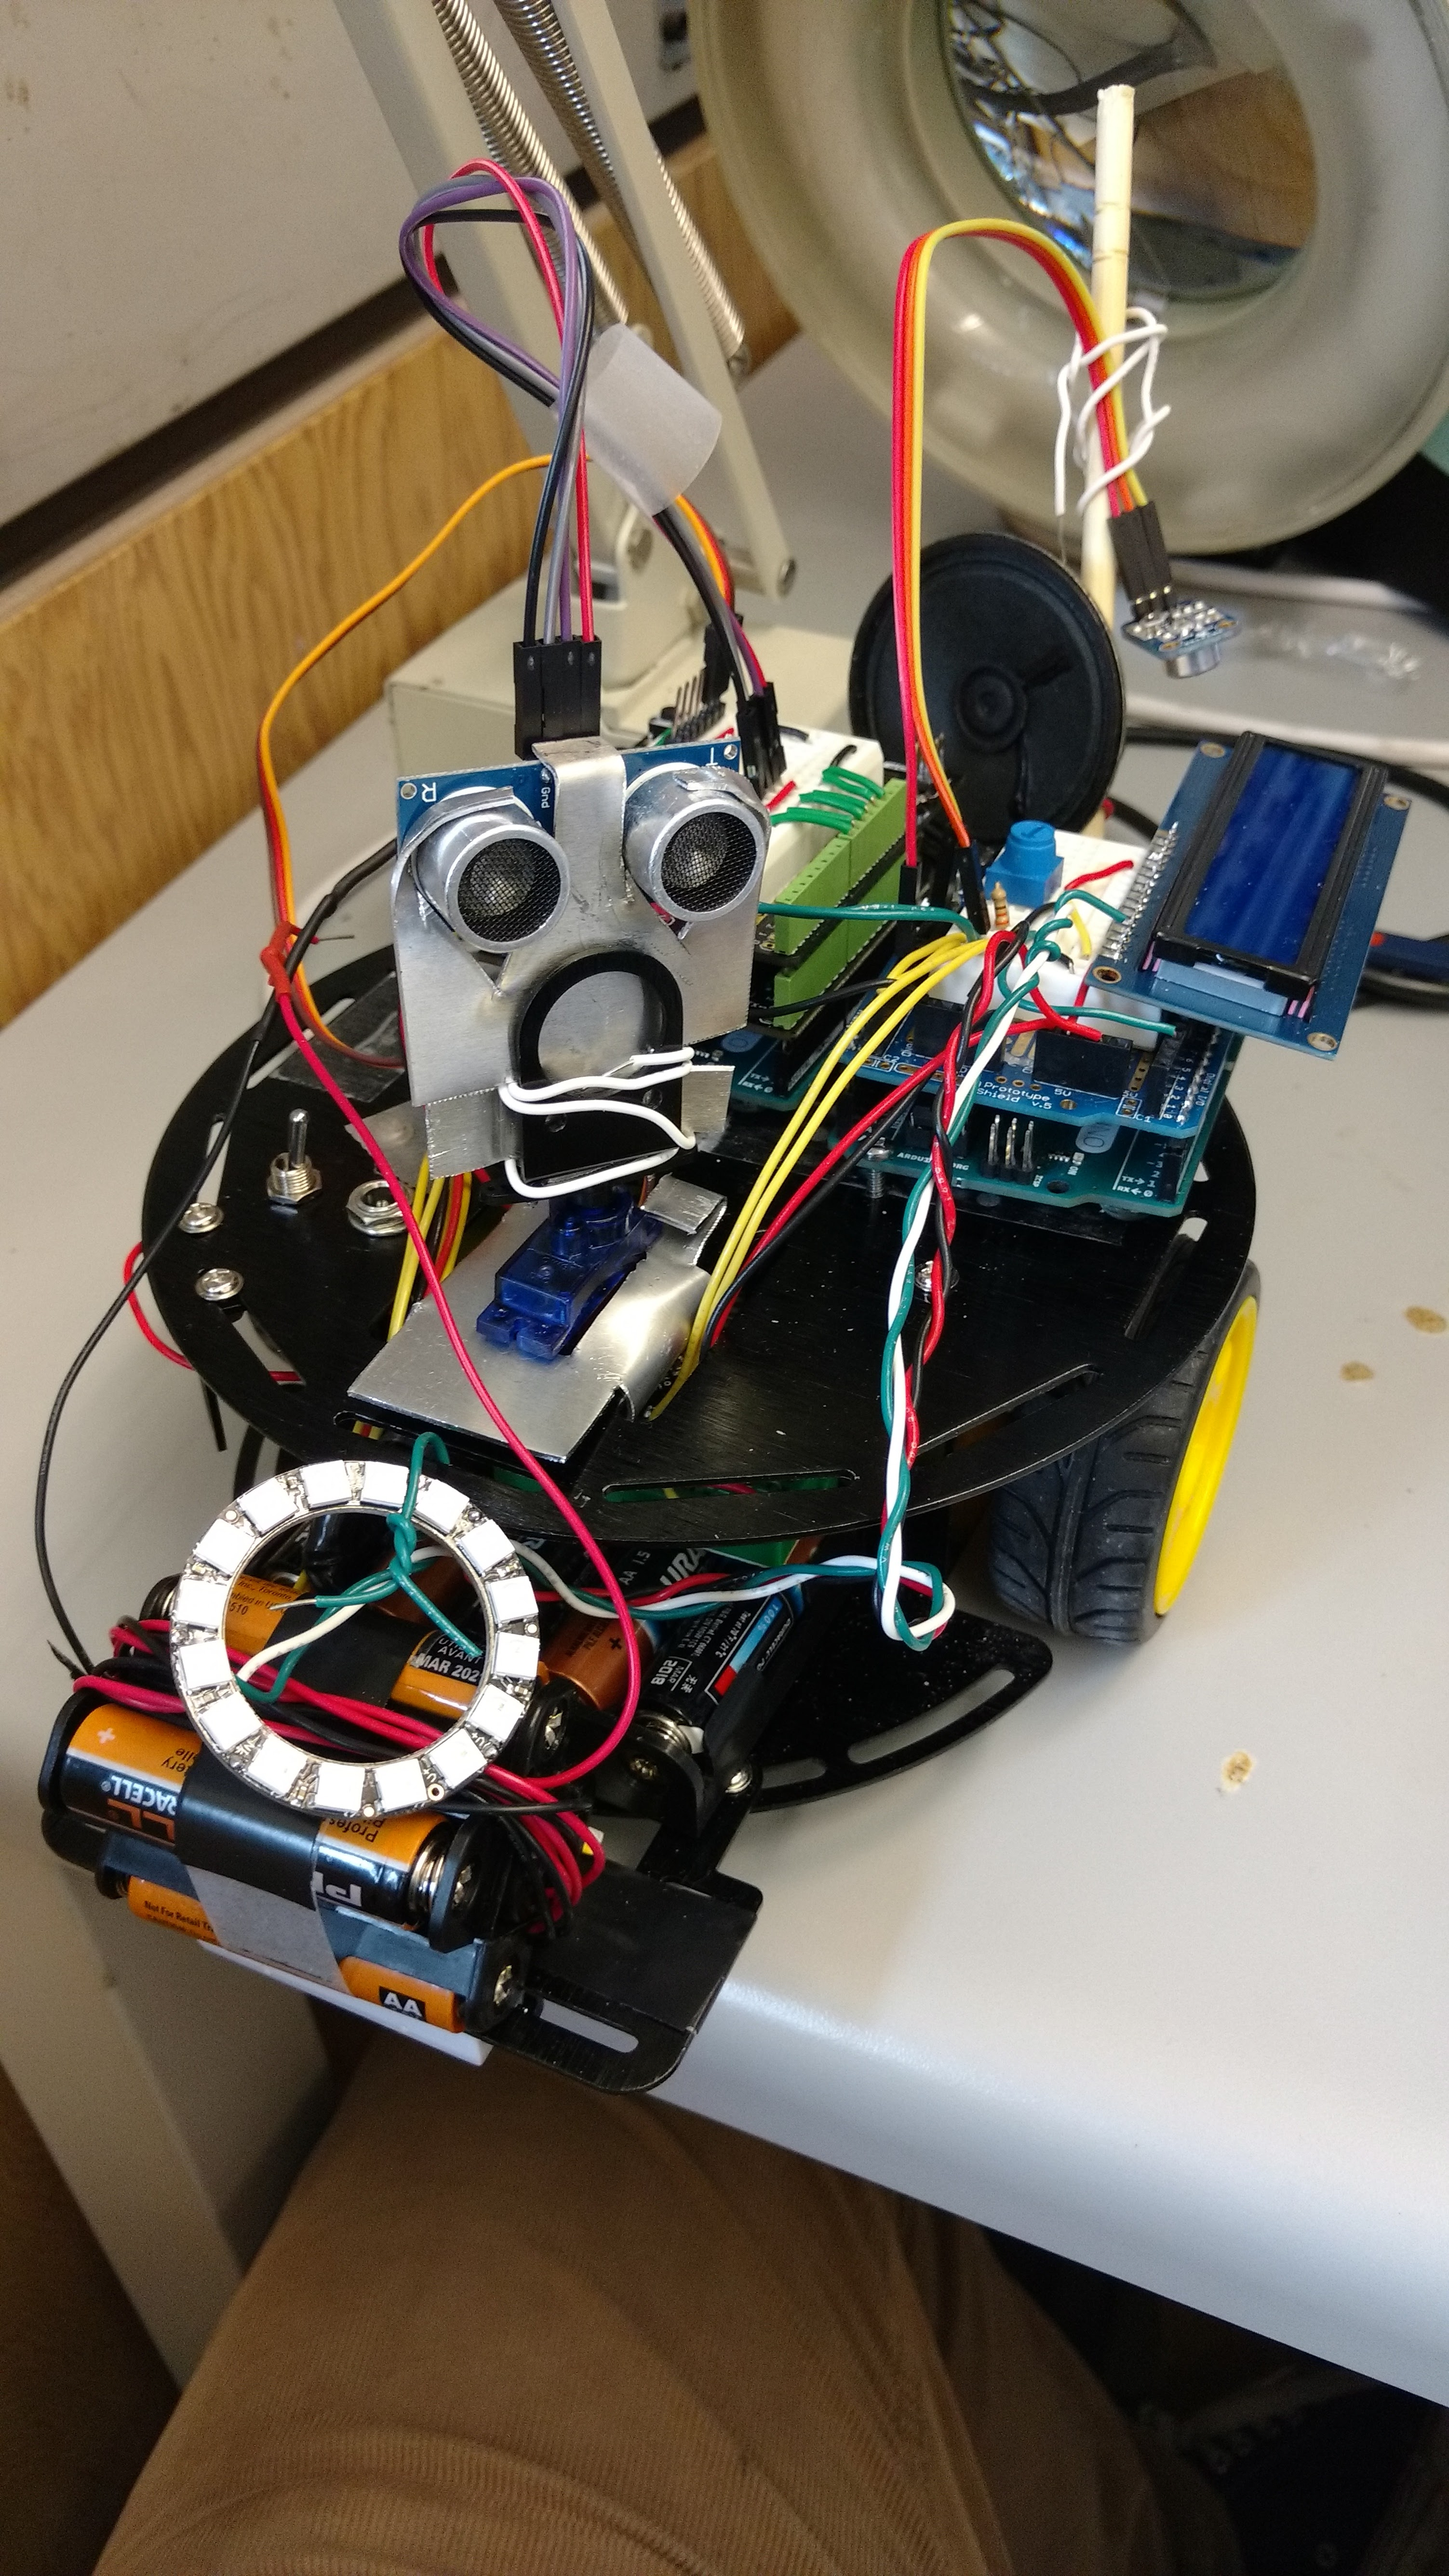
\includegraphics[width=0.35\textwidth]{1.jpg}
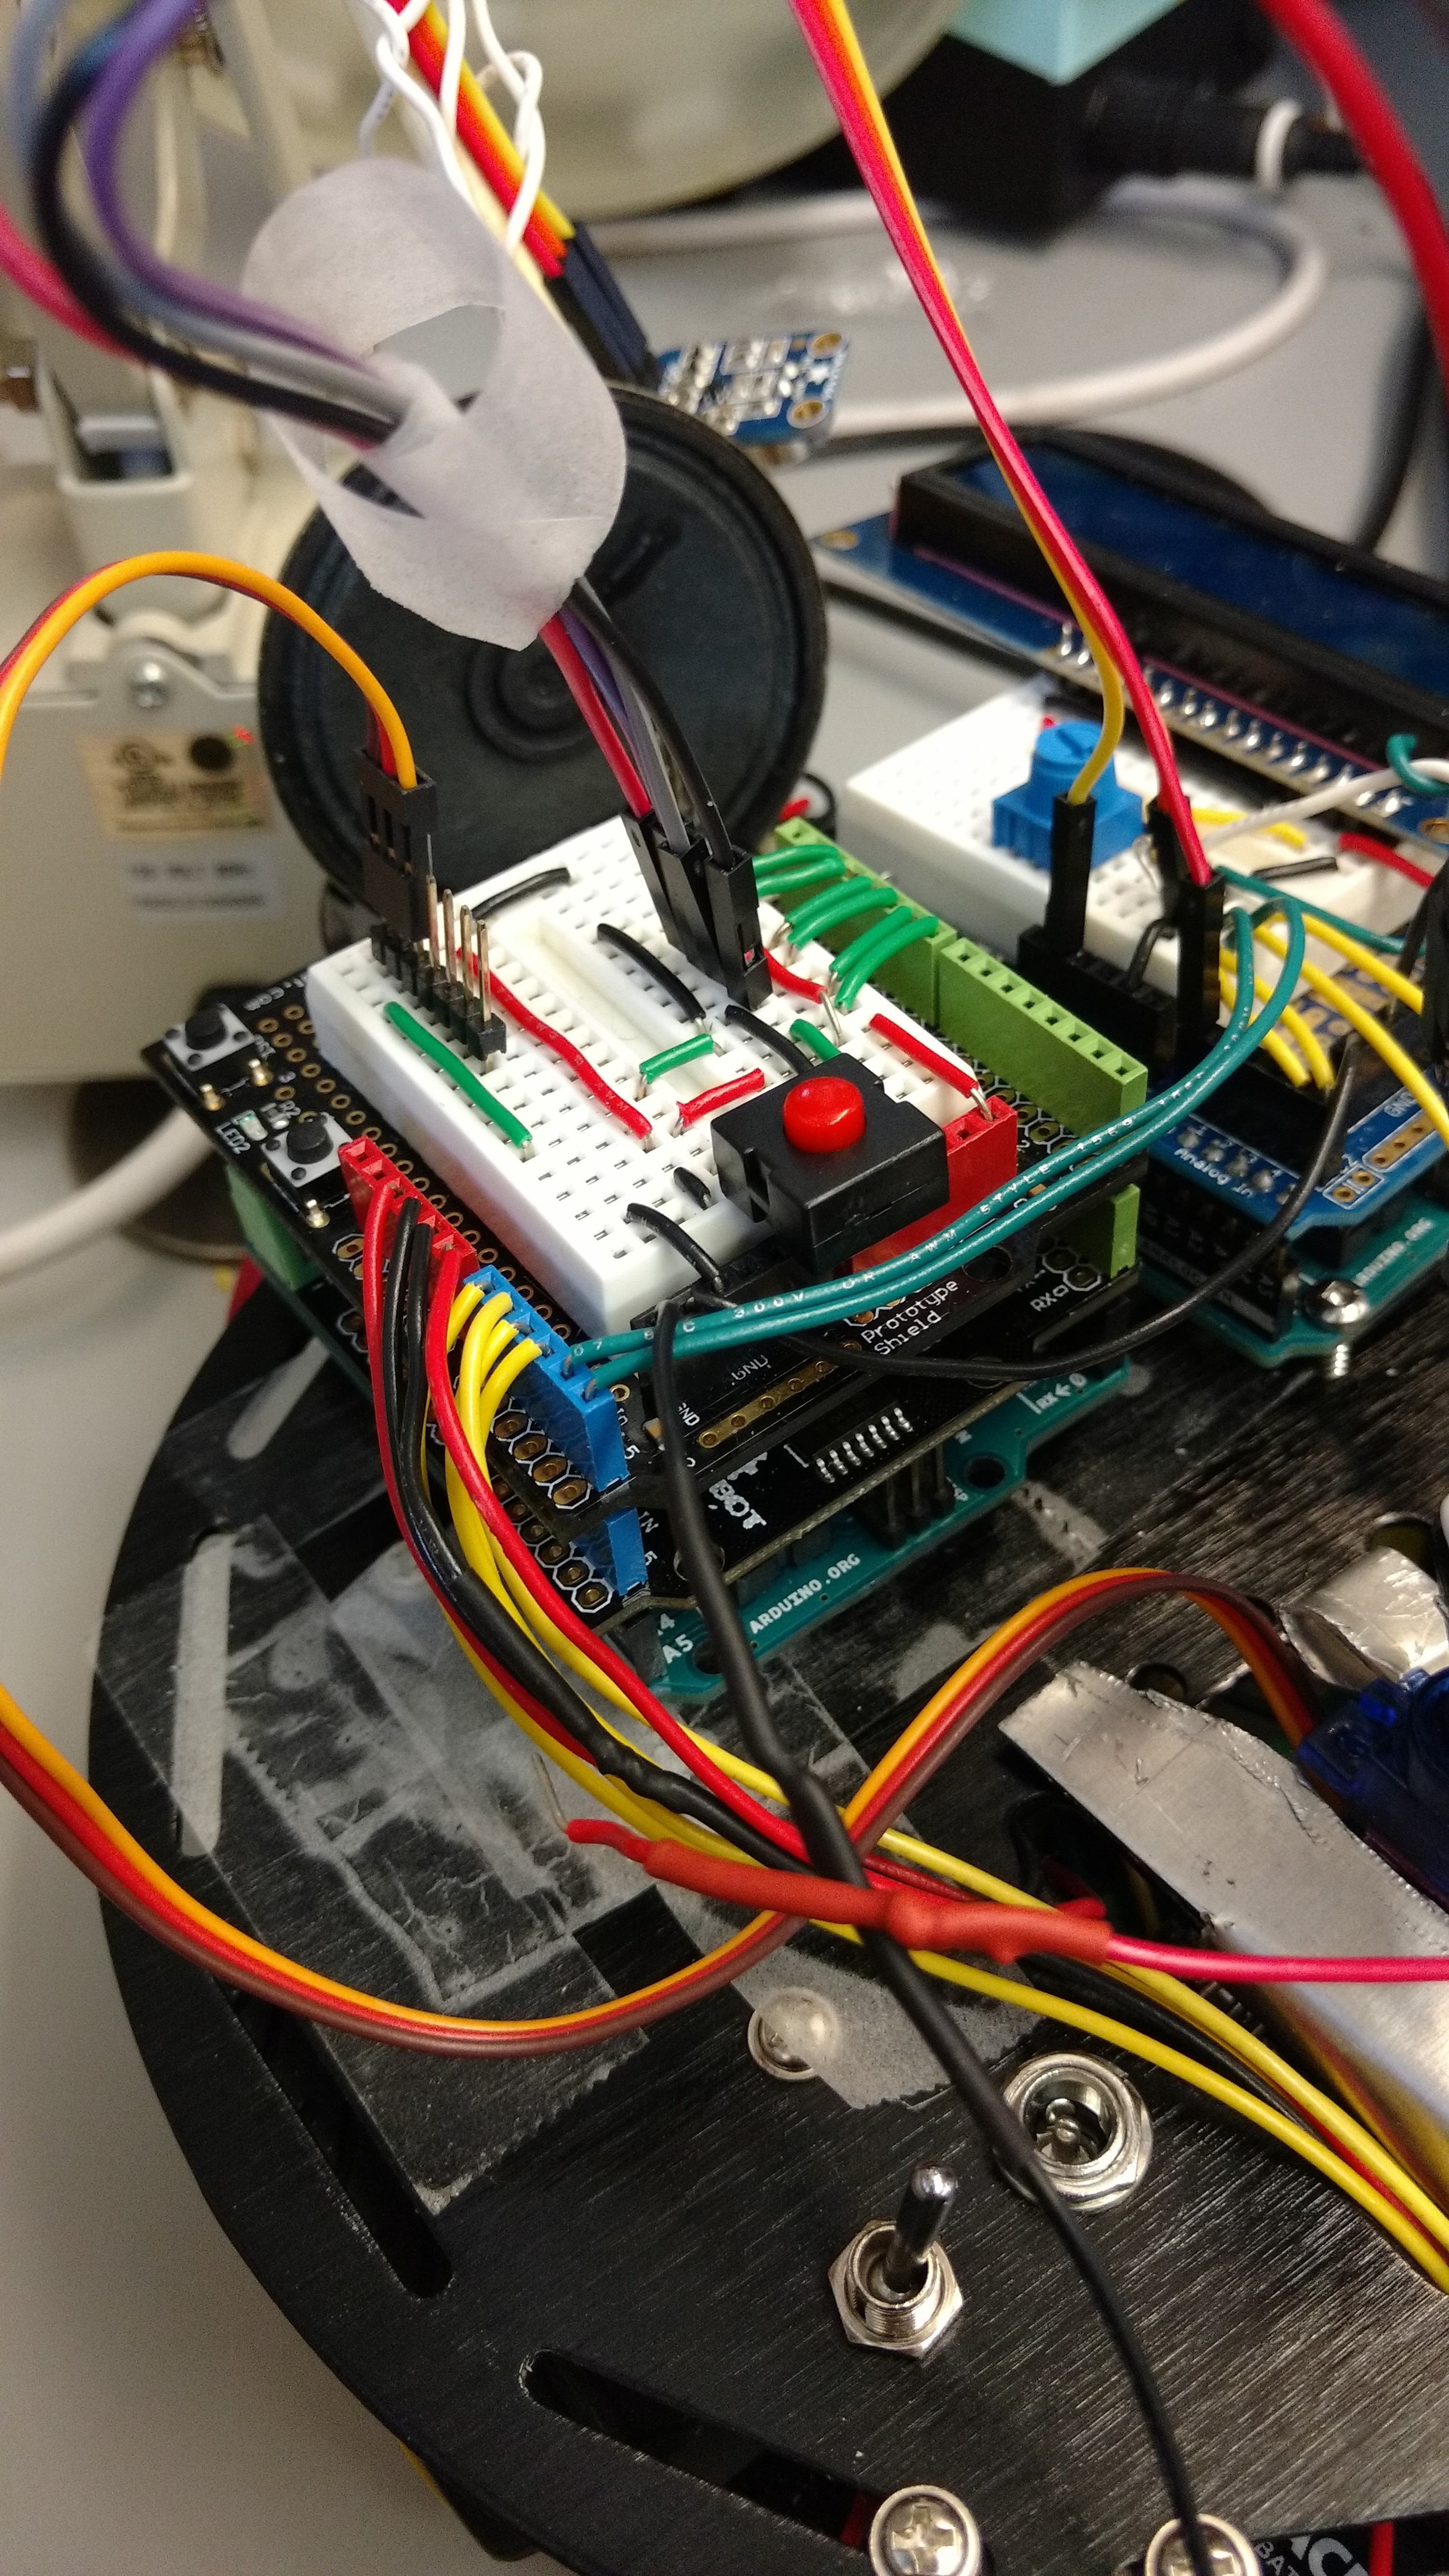
\includegraphics[width=0.35\textwidth]{2.jpg}\\
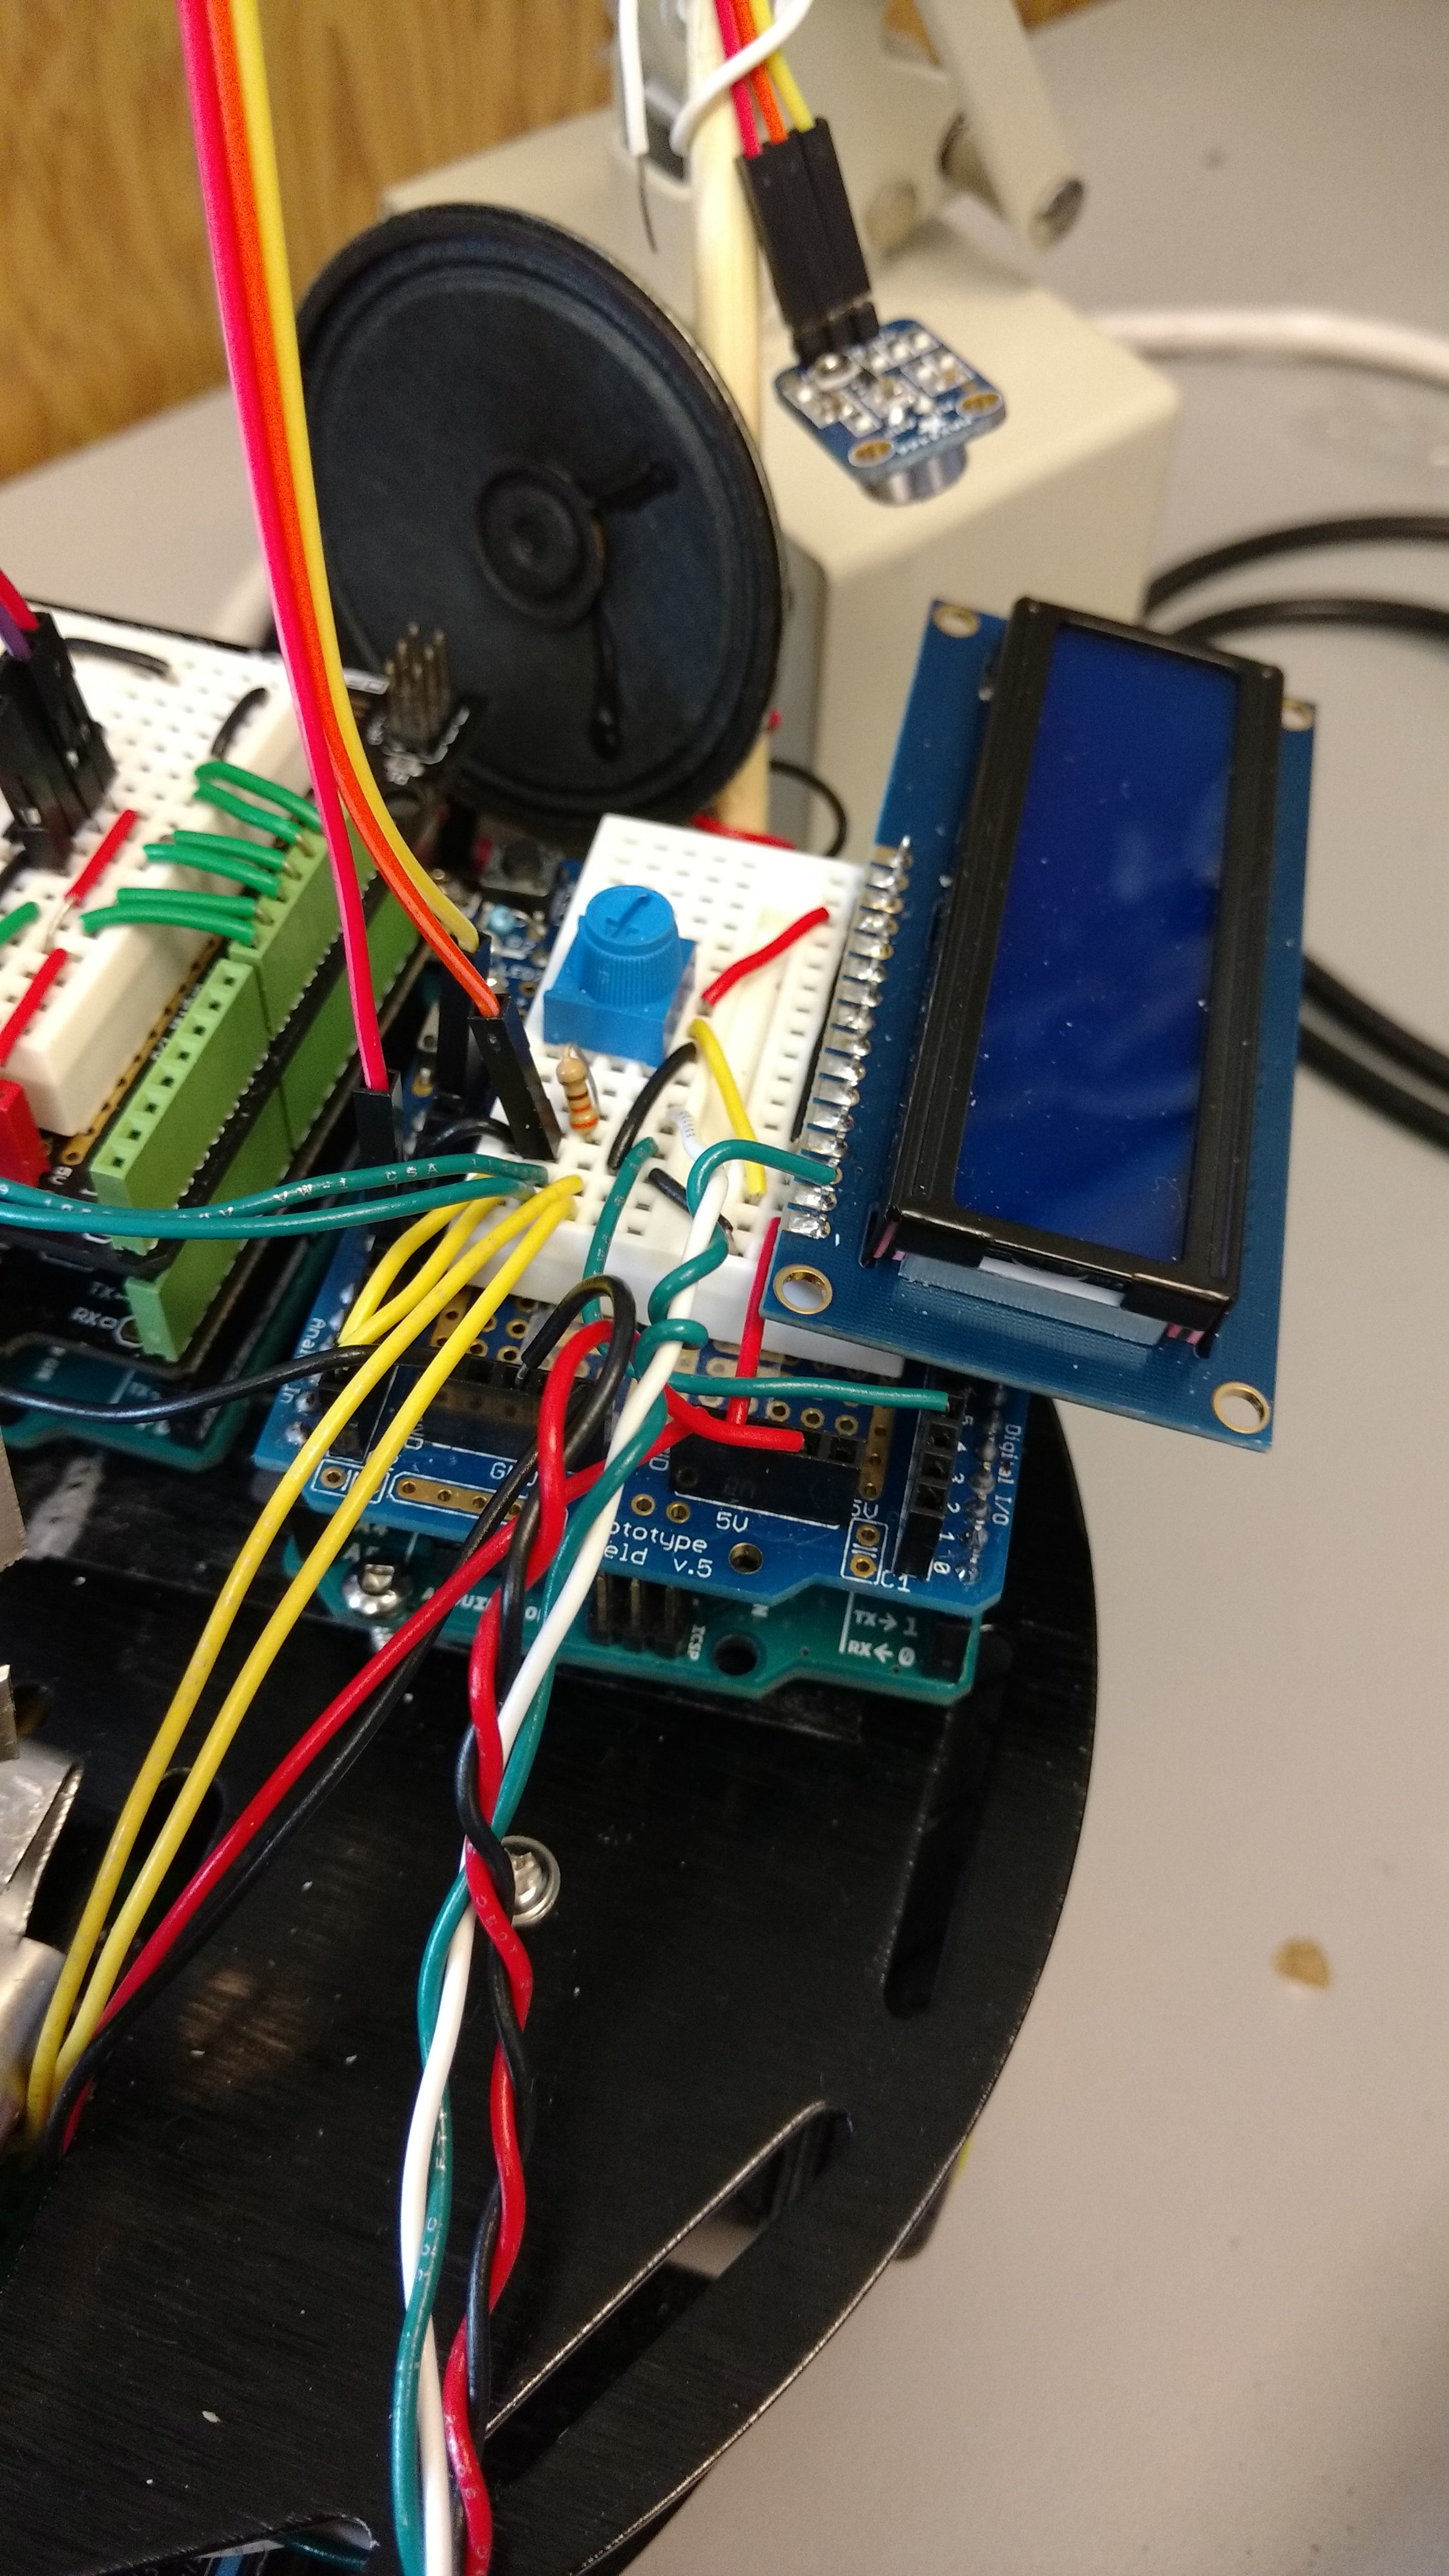
\includegraphics[width=0.35\textwidth]{3.jpg}
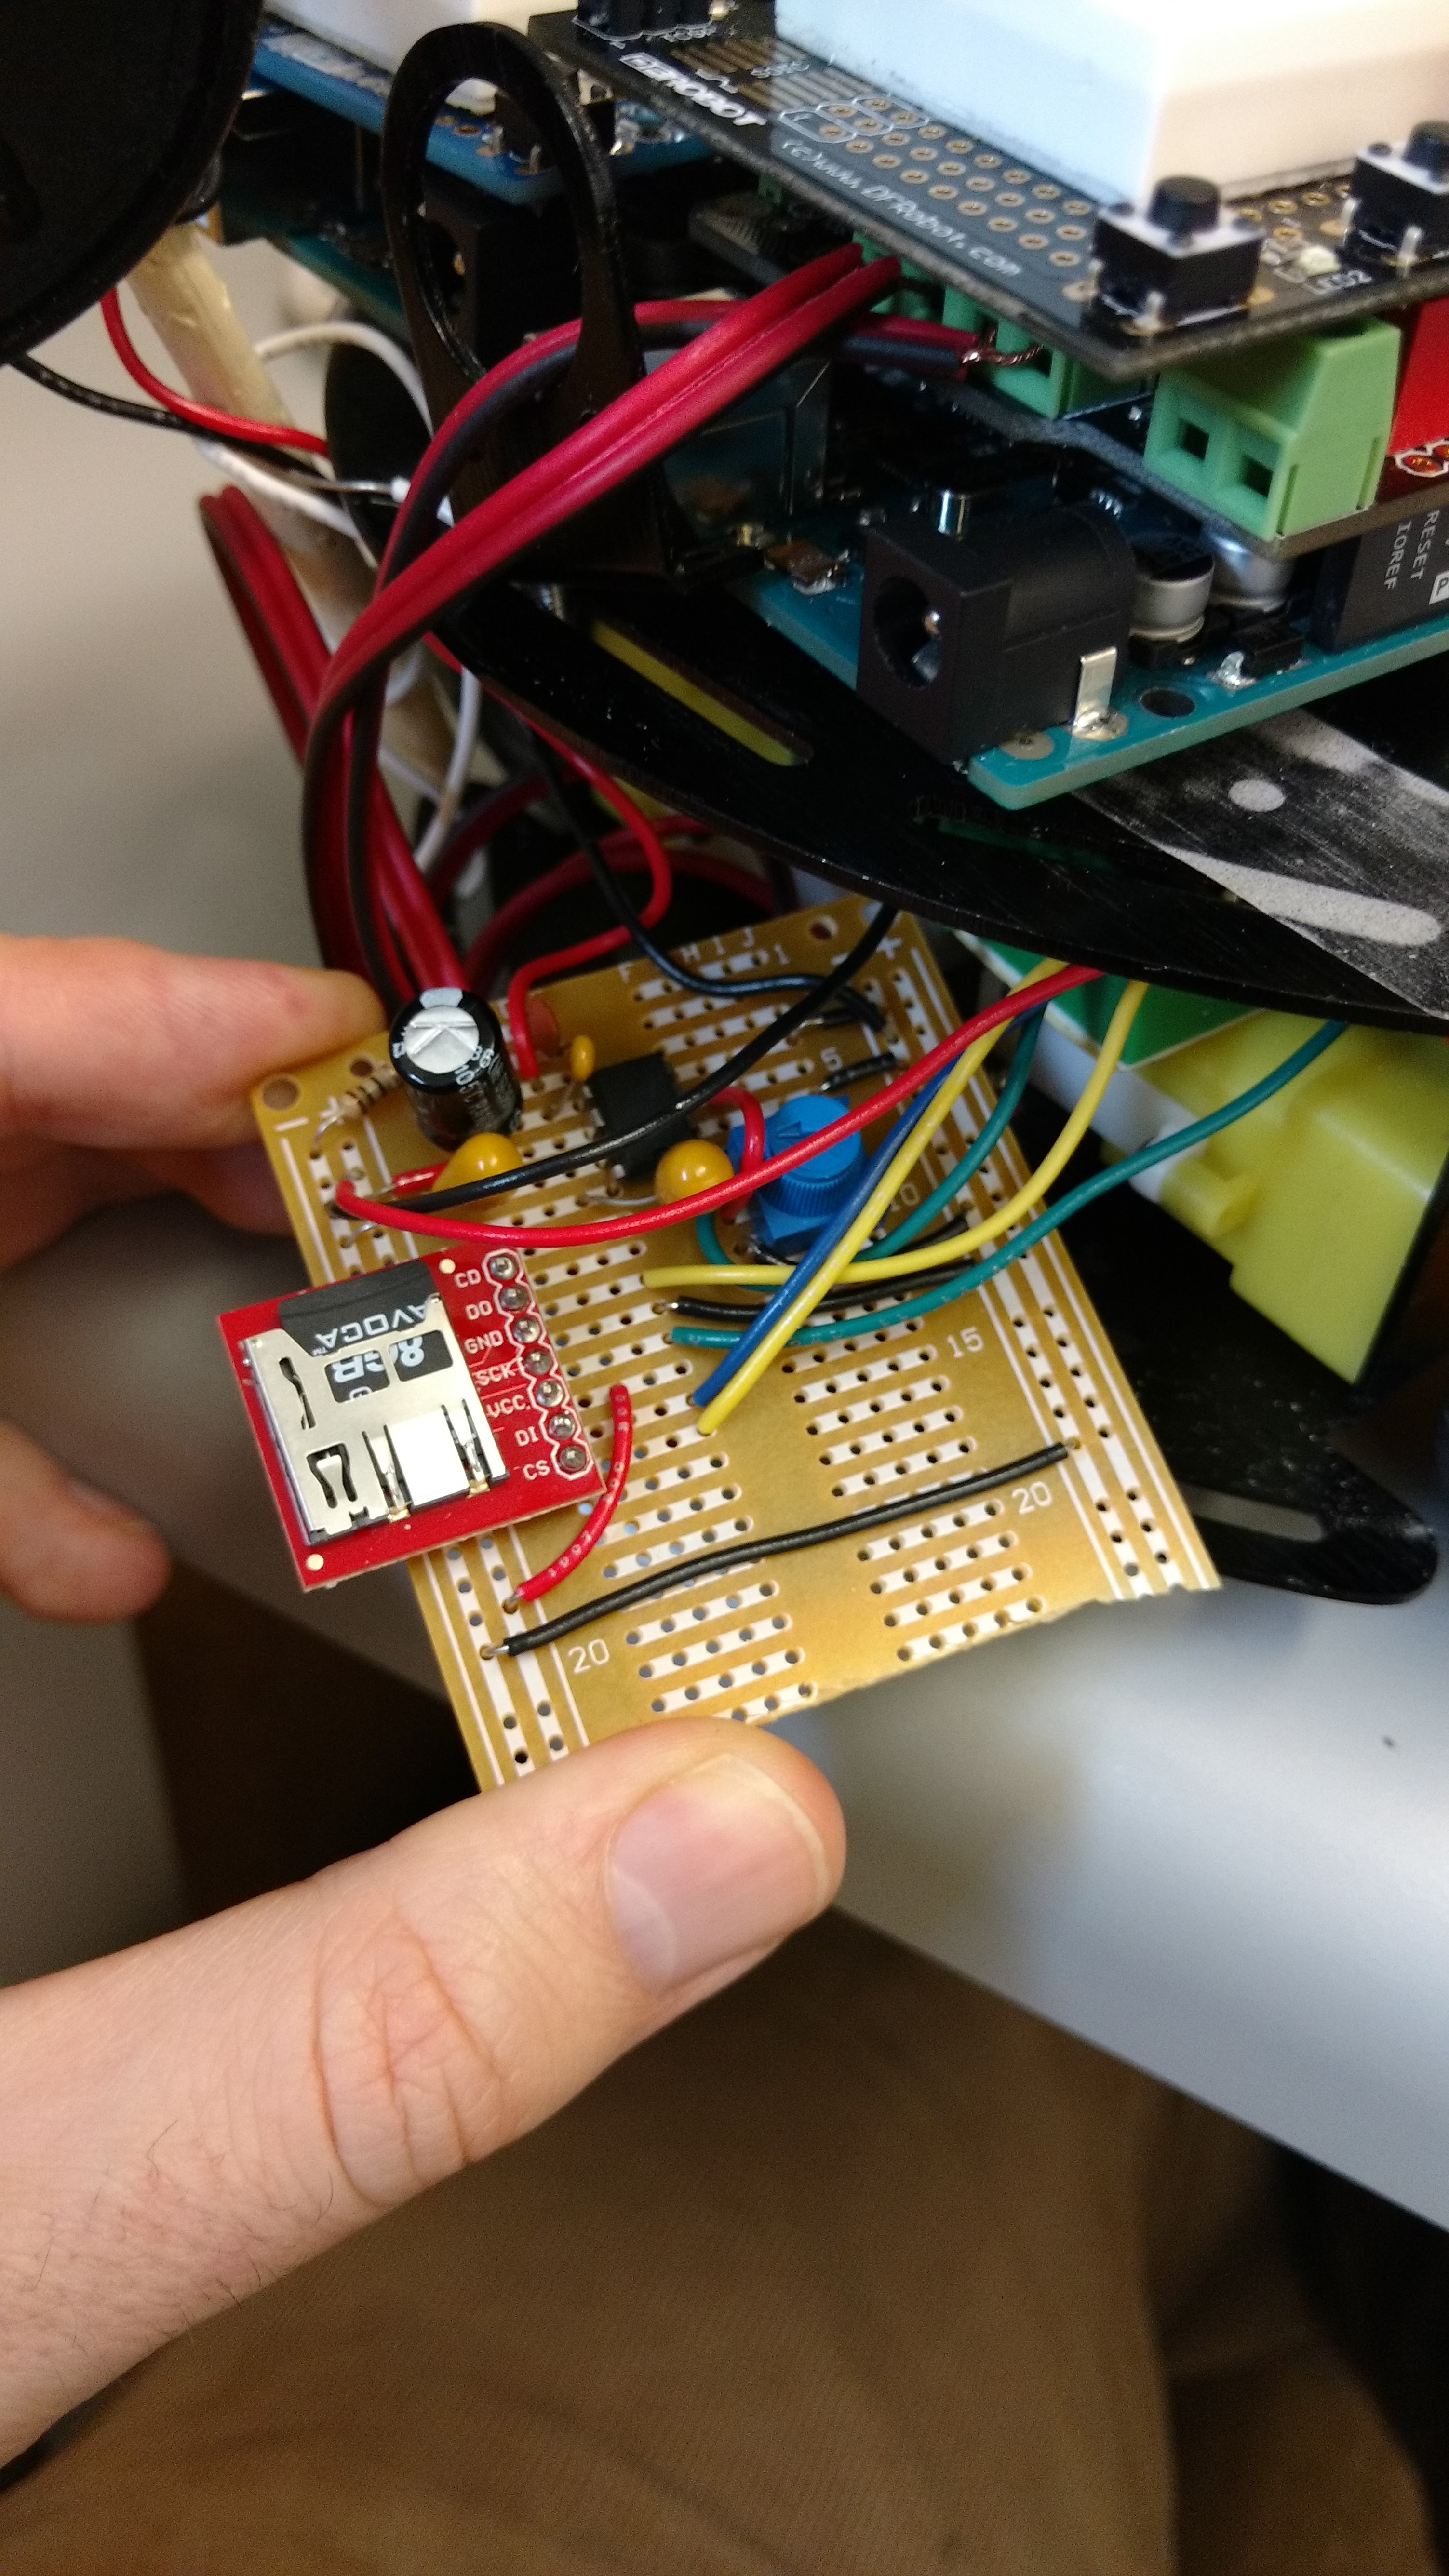
\includegraphics[width=0.35\textwidth]{4.jpg}
\newpage
\section{Appendix B - Code}
\subsection{MAIN FUNCTIONALITY: Robot.h}
\begin{verbatim}
//
//  robot.h
//  
//
//  Created by Jordan Jeffries on 2/12/16.
//
//

#ifndef robot_h
#define robot_h

#include <Servo.h>
#include <limits.h>

// max speed in cm/s
#define MAX_SPEED 61
#define DEBUG 1

// address of the slave arduino we care about on the wire bus
#define WIRE_DEVICE_1 8
#define WIRE_DEVICE_2 9
#define WIRE_TEMP_DEVICE 8

// minimum and maximum distances to be read from the ultrasonic sensors, in cm
#define DIST_MAX 100
#define DIST_MIN 0

class AI;
class ExternalData;
class Control;

/*
* struct Vector
*
* Members:
* float x: the x-component of the vector in centimetres.
* float y: the y-component of the vector in centimetres.
*/
typedef struct {
	float x;
	float y;
} Vector;

/* struct State
*
* Structure to hold state variables.
*
* float x:       the x-component of the state coordinate in cm
* float y:       the y-component of the state coordinate in cm
* float heading: the heading of the craft. Measured in radians
*                from the x-axis.
* float v:       the velocity of the robot in cm/s
* float w:       the angular velocity of the robot in rad/sec.
*
*/
typedef struct {
	float x;
	float y;
	float heading;
	float v;
	float w;
  float dt;
  uint8_t  l_PWM;
  uint8_t  r_PWM;
} State;

/*
 * enum to define possible modes.
 */
typedef enum {
	FreeDrive,
	FollowLine,
	Uninitialized
} Mode;

typedef enum {
	Left,
	Right,
        Straight
} Direction;


class AI {
public:
	/*
	* AI(ExternalData external_data, Control control)
	*
	* Initializes the AI and performs necessary setup. This function must be
	* called before any other functions.
	*
	* Parameters:
	* ExternalData external_data:  An ExternalData object from which necessary
	*                              data from the outside world will be read.
	* Control control:             A Control object with which the AI will
	*                              execute decisions that are made.
	*/
	AI(ExternalData *externalData, Control *control);
	~AI();
    
	/*
	* void decide()
	*
	* Decides what action the robot should take, and execute it.
	* This function will gather the necessary data, and then
	* execute the appropriate action.
	*/
	void decide(State *state);

private:

/*
 * Pan the servo motor from 0 to 180 
 * and return the direction corresponding to the best direction 
 * corresponding to the furthest distance read (0 degrees being 
 * left of forward relative to heading of robot, 180 being right).
 */
  Direction sweep();

  /*
   * Pan the servo motor from 0 to 180 in offset increments
   * and return the direction corresponding to the best direction 
   * corresponding to the furthest distance read (0 degrees being 
   * left of forward relative to heading of robot, 180 being right).
   */
  Vector *sweep(uint8_t offset);
	
	/*
	 * void updateMode()
	 * 
	 * Update the mode, and take any action necessary to react to the
	 * mode changing.
	 */
	void updateMode();

#pragma mark Private instance variables
	Control *_control;
	ExternalData *_externalData;
	Mode _currentMode;
  unsigned long timeSinceLastRandomSweep;
};

/*
* class Control
*
* Implements logic to output control instructions to the appropriate components.
*/
class Control {
public:
	/*
	* Control(SensorData sensor_data)
	* 
	* Initializes the object and performs necessary setup. This function
	* must be called before any other functions.
	*
	* Parameters:
	* uint8_t in1:                 The pin to which the in1 pin of the motor
	*                              shield is connected.
	* uint8_t in2:                 The pin to which the in2 pin of the motor
	*                              shield is connected.
	* uint8_t in3:                 The pin to which the in3 pin of the motor
	*                              shield is connected.
	* uint8_t in4:                 The pin to which the in4 pin of the motor
	*                              shield is connected.
    * uint8_t rangeFinder          The pin to which the servo controlling the
    *                              range finder is connected.
	*/
	Control(uint8_t rangeFinder);
	~Control();
    
    /*
     * void initializePins()
     *
     * Sets Arduino pin modes. This method should be called from setup() and before
     * any other functions.
     */
    void initializePins();
    
    /* 
     * void setExternalData(ExternalData *externalData)
     *
     * Set the ExternalData object form which data about the outside world
     * should be collected.
     */
    void setExternalData(ExternalData *externalData);
        
	/*
	* go(Vector direction, bool stopAtDestination)
	*
	* Causes the robot to proceed in the direction specified by direction.
	* 
	* Parameters:
	* vector destination:      A vector specifying the direction in which
	*                          the robot should travel. The origin of the
	*                          vector is assumed to be the center of the
	*                          robot.
	* bool stopAtDestination:  (REMOVED, OPTIONAL). Defaults to false.
	*                          Specifies whether the robot should stop once
	*                          it reaches the point specified by direction.
	*                          If false, the robot will continue in the
	*                          specified direction until instructed otherwise.
	*
	*/
	void go(State *state, Vector *destination, bool stopAtDestination);
    
	/*
	* void stop()
	*
	* Causes the robot to cease all movement immediately.
	*/
	void stop();
    
	/*
	* void orientRangeFinder(int orientation)
	*
	* Causes the ultrasonic range finder on the rotatable platter to
	* assume the specified orientation.
	*
	* Parameters:
	* int orientation: The orientation the range finder should assume,
	*                  specified in degrees. The value should be in the
	*                  range of 0 to 359, inclusive. 0 degrees will be
	*                  assumed be the straight ahead, 90 straight to
	*                  the right, 180 straight back, and 270 straight
	*                  to the left. See the figure below for details.
	*
	*                  0
	*      315 -----------------  45
	*         |      front      |
	*         |                 |
	*         |        ^        |
	*         |       / \       |
	*         |        |        |
	*     270 |      <-+->      | 90
	*         |        |        |
	*         |       \ /       |
	*         |        ˇ        |
	*         |                 |
	*         |      back       |
	*      225 -----------------  135
	*                 180
	*/
	void orientRangeFinder(int orientation);

        /*
         * Decrease the speed the robot is moving at by a small amount.
         */
          void slowDown(State *state);
      
        /*
         * Attached the servo motor to its designated input pin.
         */
        void attachRangeFinder();
	
	/*
	 * Send a byte to the slave Arduino to indicate that it should 
	 * take some action.
	 */
	void sendByteToSlave(char byte);

        /*	void adjustHeading(State * state, Vector * destination);	
	*
	*	Caculates an error in its heading, and stabilizes it to zero by adjusting wheel speeds.
	*	
	*	Parameters:		
	*	State * state:          The state structure. Pre-loaded is a current heading. 
	*				
	*	Vector * destination:	A vector structure with a desired destination.
	*		
	*/	
        void adjustHeading(State * state, Vector * destination, bool hard);
    
private:
	/*	void wheelControl(float right_velocity, float left_velocity)
	*
	*	Applies PWM signal to wheel motors. Must convert velocities into
	*   PWM appropriate signal (integer from 0-255)
	*	
	*	Parameters:
	*	float left_w:		  An angular velocity, specified in radians
	*						  per second, to be applied to the left wheel.
	*						  This function will assume velocities requested
	*						  are within the operating range of the motor as 
	*						  specified in the datasheet. This function must 
	*						  convert the angular velocity to some integer 
	*						  between 0 & 255 using a linear model.
	*
	*	float left_w:		  An angular velocity, specified in radians per
	*						  second, to be applied to the right wheel. Similar
	*						  conditions to the left_w parameter.
	*/
	void wheelControl(State * state, bool left, bool right);

	/*	void calculateOdometry(State * state, float left_w, float right_w)
	*
	*	Calculates distance travelled in an individual time step and updates the 
	*	state variables to match. Should be called following each time step so that
	*	the state variables in the x-y plane and the heading remain up to date.
	*	
	*	Parameters: 
	*	State * state:		A pointer to the state structure.
	*	float left_w:		(Read "left omega"). The angular velocity of the left 
	*						during the time step.
	*	float right_w:		(Read "right omega") The angular velocity of the right
	*						wheel during the time step.
	*/
	void calculateOdometry(State * state, float left_w, float right_w);
   
	/*	float wheelVelocity(float w, float v, int wheel)	
	*
	*	Computes left or right wheel angular velocity given craft desired velocity
	*  	and angular velocity. Documentation on these formulae is availabile in the
	*	accompanying report. This abstraction allows us to use a unicycle dynamical
	*	model instead of a differential drive when making incremental state changes.
	*	
	*	Parameters:		
	*	float w:		("omega") A desired angular velocity of the robot, for one 
	*					time step.
	*	float v:		A desired velocity of the robot, for one time step.
	*		
	*	Returns:		A wheel velocity in float format for the wheelControl function
	*					to apply to the wheels, and for the calculateOdometry function
	*					to use in calculating state changes during a time step.
	*/	
	float wheelVelocity(float w, float v, int wheel);
 
public:
 /*	void followLine(float *reflectivities)	
	*
	*	Completes one time step in the control flow of a line-following behaviour.
	*	
	*	Parameters:		
	*	State *state:	 state variable representing the action to be taken by
	* 							 the robot.
	*/	
  void followLine(State *state);
    
private:
#pragma mark Pin instance variables
    uint8_t rangeFinderPin;
    
#pragma mark Servo instance variables
    Servo rangeFinderServo;
		int _currentRangeFinderOrientation;
		
#pragma mark Slave command instance variables
		char _last_command;
};

/*
* class ExternalData
*
* Implements logic to acquire data from input devices. This class may use caching
* in order to reduce actual accesses to hardward devices. Every data acquisition
* method will specify its caching behaviour.
*/
class ExternalData {
public:
	// these constructors are subject to change
	/*
	* ExternalData(int temperaturePin, int numberOfUltrasonicSensors, int* ultrasonicSensors)
	*
	* Initializes ExternalData and performs necessary setup. This function
	* must be called before any other functions.
	*
	* Parameters:
	* int numberOfUltrasonicSensors:   the number of ultrasonic sensors that are
	*                                  available to the robot.
	* uint8_t** ultrasonicSensors:     pins to which each ultrasonic sensor is connected.
	*                                  The array should be formatted as follows, indexed
	*                                  as ultrasonicSensors[index]:
	* 
	*          index   value
	*          0       pin to which the trigger pin of the 0th ultrasonic
	*                  sensor is connected.
	*          1       pin to which the echo pin of the 0th ultrasonic sensor
	*                  is connected.
	*          2       pin to which the trigger pin of the 1st ultrasonic
	*                  sensor is connected.
	*          3       pin to which the echo pin of the 1st ultrasonic sensor
	*                  is connected.
	*
	*                                   And so on.
    * int numberOfReflectivitySensors:  The number of reflectivity sensors that are
    *                                   available to the robot.
    * uint8_t* reflectivitySensors:     Pins to which the reflectivity sensors are
    *                                   connected.
	*/
	ExternalData(int numberOfUltrasonicSensors, uint8_t ultrasonicSensors[], int numberOfReflectivitySensors, uint8_t reflectivitySensors[], int mode_pin);
	~ExternalData();
  
	/*
	 * void initializePins()
	 *
	 * Sets Arduino pin modes. This method should be called from setup() and before
     * any other functions.
	 */
	void initializePins();
    
	/*
	* void clearCache()
	*
	* Instructs the class to clear its data cache. Values returned immediately
	* after this method is called will always query sensors.
	*/
	void clearCache();
    
	/*
	* float temperature(bool fresh)
	* 
	* Returns the current ambient air temperature in degrees Celsuis. This function
	* may perform caching.
	*
	* Parameters:
	* bool fresh:  This parameter is optional.
	*              If true, the cache will be ignored and fresh data will be
	*              read from the appropriate sensors.
	*/
	float temperature(bool fresh = false);
    
	/*
	* float distance(bool fresh)
	*
	* Returns the current distance to the nearest object as seen by an ultrasonic
	* range finder in cm. This function may perform caching.
	*
	* Parameters:
    * int sensor:        ultrasonic sensor from which to read distance
	* bool fresh:  		 if true, the cache will be ignored and fresh data will be
	*              		 read from the appropriate sensors.
	*/
	float distance(int sensor, bool fresh = false, int maxChange = INT_MAX);
    
	/*
	* float* distances(bool fresh)
	* 
	* Returns the current distance to the nearest object in line of sight as seen by each ultrasonic
	* range finder. The units of the return value will be the same as the distance()
	* function. The return array will be indexed as follows:
	*
	*          index   value
	*          0       distance from sensor 0 to nearest object
	*          1       distance from sensor 1 to nearest object
	*          2       distance from sensor 2 to nearest object
	*
	* and so on. The value returned by this function will be dynamically allocated,
	* and must be freed by the caller.
	*
	* This function may perform caching.
	*
	* Parameters:
	* bool fresh:  	if true, the cache will be ignored and fresh data will be
	*              	read from the appropriate sensors.
	*/
	float* distances(bool fresh = false);
    
	/*
	* float reflectivity(int sensor, bool fresh)
	*
	* Returns the reflectivities seen by the reflective optical sensors. This function
	* may perform caching.
	* 
	* Parameters:
	* int sensor:  the sensor to read reflectivity from 
	* bool fresh:  if true, the cache will be ignored and fresh data will be
	*              read from the appropriate sensors. Defaults to false.
	*/
	float reflectivity(int sensor, bool fresh = false);
	
	/*
	* float *reflectivities(bool fresh)
	*
	* Returns the reflectivities seen by the reflective optical sensors. This function
	* may perform caching.
	* 
	* Parameters:
	* bool fresh:  if true, the cache will be ignored and fresh data will be
	*              read from the appropriate sensors.
	*/
	float *reflectivities(bool fresh = false);

 /*
  * Get the mode the robot is currently in by reading from a push-button
  * Returns 0 if the button is pressed corresponding to LINE_MODE for 
  * following a line on the ground, or returns 1 if the button is not 
  * pressed curresponding to FREE_DRIVE_MODE for driving around freely.
  */
  Mode mode();

  float read_temperature();
  float readDistance(int sensor, float temperature);

 
private:
#pragma mark Pin variables
	int _temperaturePin;
  int _modePin;
	int _numberOfUltrasonicSensors;
	uint8_t* _ultrasonicSensorPins;
  int _numberOfReflectivitySensors;
  uint8_t* _reflectivitySensorPins;
    
#pragma mark Caching variables
	float _lastTemperature;
	float *_lastDistances;
	float *_lastReflectivities;
    
	unsigned long _lastTemperatureTimestamp;
	bool *_distancesCached;
	bool *_reflectivitiesCached;
    
#pragma mark Data acquisition functions
	float _readTemperature();
	void _pulseOut(uint8_t pin, int microseconds);
	float _readDistance(int sensor, float temperature);
};

#endif /* robot_h */

\end{verbatim}

\subsection{MAIN FUNCTIONALITY: Robot.ino}
\begin{verbatim}
#include <Wire.h>

#include <Servo.h>

#include "Robot.h"

// ultrasonic sensors
#define NUMBER_OF_ULTRASONIC_SENSORS 2

// sensor 0 is mobile, sensor 1 is straight ahead
#define DIST_SENSOR_0_ECHO_PIN 10
#define DIST_SENSOR_1_ECHO_PIN 13
#define DIST_SENSOR_0_TRIGGER_PIN 11
#define DIST_SENSOR_1_TRIGGER_PIN 12

// servo to orient the rotatable distance sensor
#define SERVO_PIN 9

// mode swtich
#define MODE_SWITCH_PIN 8

// reflectivity sensors
#define NUMBER_OF_REFLECTIVITY_SENSORS 4

#define REFLECTIVITY_SENSOR_1_PIN A3 // leftmost sensor
#define REFLECTIVITY_SENSOR_2_PIN A2
#define REFLECTIVITY_SENSOR_3_PIN A1
#define REFLECTIVITY_SENSOR_4_PIN A0 // rightmost sensor

// variables required to initialize ExternalData
uint8_t ultrasonicSensorPins[4] = {
	DIST_SENSOR_0_TRIGGER_PIN, DIST_SENSOR_0_ECHO_PIN,
	DIST_SENSOR_1_TRIGGER_PIN, DIST_SENSOR_1_ECHO_PIN
};

uint8_t reflectivitySensors[4] = {
	REFLECTIVITY_SENSOR_1_PIN,
	REFLECTIVITY_SENSOR_2_PIN,
	REFLECTIVITY_SENSOR_3_PIN,
	REFLECTIVITY_SENSOR_4_PIN
};

ExternalData externalData(NUMBER_OF_ULTRASONIC_SENSORS, ultrasonicSensorPins, NUMBER_OF_REFLECTIVITY_SENSORS, reflectivitySensors, MODE_SWITCH_PIN);
Control control((uint8_t)SERVO_PIN);
AI ai(&externalData, &control);

State state;
Vector destination;

void setup() {
	// Serial.begin(9600);
	Wire.begin();
	
	externalData.initializePins();
	control.attachRangeFinder();
	control.initializePins();
	
	delay(500);
	control.sendByteToSlave('k');
	delay(1500);
 
	state.x = 0;
	state.y = 0;
	state.v = 61;
	state.w = 0;
	state.dt = 1;
	state.heading = M_PI/2;
	state.l_PWM = 0;
	state.r_PWM = 0;
	destination.x = 0;
	destination.y = 300;
  	
	control.stop();
}

void loop() {
	externalData.clearCache();
	
#ifdef DEBUG
	Mode mode = externalData.mode();

	if (mode == FreeDrive) {
		Serial.println("Free drive");
	} else if (mode == FollowLine) {
		Serial.println("Follow line");
	} else {
		Serial.println("Invaid mode");
	}
#endif
		
  ai.decide(&state);
}


\end{verbatim}

\subsection{MAIN FUNCTIONALITY: Control.ino}
\begin{verbatim}
/*
Robot differential control system
  
By Chad Lagore
02/13/16
*/

#include <math.h>
#include "Robot.h"

// pins for the motor shield
#define E1 5  
#define M1 4 
#define E2 6                      
#define M2 7 

// Geometric constants of robot vehicle.
// Wheel radius (R) and wheel to wheel length (L).
#define R 6.5
#define L 16

#define SERVO_DELAY_PER_DEGREE 3

#define _USE_MATH_DEFINES

#pragma mark Begin Control implementation

Control::Control(uint8_t receivedRangeFinder) {
	rangeFinderPin = receivedRangeFinder;
}

Control::~Control() {
	// TODO: implement
}

void Control::initializePins() {
	pinMode(E1, OUTPUT);
	pinMode(E2, OUTPUT);
	pinMode(M1, OUTPUT);
	pinMode(M2, OUTPUT);
	pinMode(rangeFinderPin, OUTPUT);

}

void Control::attachRangeFinder() {
	rangeFinderServo.attach(rangeFinderPin);
}


/*  go(State state, Vector destination, bool StopAtDestination = false)
    
Control flow for a single time step in moving the robot towards its
destination. 
*/
void Control::go(State * state, Vector * destination, bool stopAtDestination) {
	float distance, MAX_RPM;
	state->heading = M_PI/2;
	MAX_RPM = 160.0;
	float factor = 8.0;
        
        /* Adjust heading */
        adjustHeading(state, destination, false);
        
	/* Determine desired distance */
	distance = sqrt(destination->x*destination->x + destination->y*destination->y);
	
	/* Implement desired wheel speeds */
	state->l_PWM = state->v / MAX_SPEED * 255;
	state->r_PWM = state->v / MAX_SPEED * 255;
	wheelControl(state, true, true);
        
	/* Drive straight  */
        if(stopAtDestination) {
      	    while(distance > 2) {
      		distance = distance - (factor * MAX_RPM / 60000 * 2 * R * M_PI/2);
      		delay(10);
      	    }
            stop();
        }
        
}

/*  Applies PWM signal to wheel motors. This function will require access
*  to pin numbers.
*/
void Control::wheelControl(State * state, bool left, bool right) {
        digitalWrite(M1, right ? HIGH : LOW); 
        digitalWrite(M2, left ? HIGH : LOW);
        analogWrite(E1, state->r_PWM); 
        analogWrite(E2, 0.98*state->l_PWM);
}

void Control::adjustHeading(State * state, Vector * destination, bool hard) {
        float desired_heading, error, arc, MAX_RPM;
	MAX_RPM = 160.0;
	float factor = 10.0;
        state->heading = M_PI/2;
        
	arc = 3.0 * MAX_RPM / 60000 * 2 * M_PI * R * 2;
        arc = hard ? arc : arc / 2;
        
	/* Determine desired heading, velocity and angular velocity */
	desired_heading = atan2(destination->y, destination->x); 
	error = state->heading - desired_heading;
	error = atan2(sin(error), cos(error));
	// Serial.println(error);
        
	/* Correct heading */
	while(abs(error) > 0.05) {
                if(hard) {
                    state->l_PWM = 255;
		    state->r_PWM = 255;
		    wheelControl(state, error < 0, error > 0);
                }
                else { 
                    state->l_PWM = error < 0 ? 0 : 255;
                    state->r_PWM = error > 0 ? 0 : 255;
                    wheelControl(state, true, true); 
                }
		delay(10);
		state->heading = (error > 0) ? state->heading - arc/L : state->heading + arc/L;
		error = state->heading - desired_heading;
		error = atan2(sin(error), cos(error));
		// Serial.println(error);
	}
}

/*
* Set the servo motor to point in the direction 
* specified by the orientation parameter.
*/
void Control::orientRangeFinder(int orientation) {
	if (_currentRangeFinderOrientation != orientation) {
		rangeFinderServo.write(orientation);
		// give the servo a chance to actually move - 3ms per degree moved
		delay(SERVO_DELAY_PER_DEGREE * abs(_currentRangeFinderOrientation - orientation));
		_currentRangeFinderOrientation = orientation;
	}
}
/*
*  Completes one time step in the control flow of a line-following behaviour.
*/
void Control::followLine(State * state) {
	const float factor = 2.0;
	digitalWrite(M1, HIGH); digitalWrite(M2, HIGH);
	analogWrite(E1, factor*state->l_PWM); analogWrite(E2, factor*state->r_PWM);
}

void Control::stop() {
	digitalWrite(M1, HIGH); digitalWrite(M2, HIGH);
	analogWrite(E1, 0); analogWrite(E2, 0);
}

void Control::slowDown(State *state) {
	state->v = state->v - 2;
	
	if (state->v < 25) {
		state->v = 25;
	}
	
	// Serial.print("New velocity: ");
	// Serial.println(state->v);
	
	Vector destination;
	destination.x = 0;
	destination.y = 1;
	go(state, &destination, false);
	//decrement current wheel speed by some about and write this new value back to the wheels
}

void Control::sendByteToSlave(char command) {
	if (command == _last_command) {
		if (command == 'b' || command == 'd') {
			return;
		}
	}
	
	_last_command = command;
	
	// write to the first device
	Wire.beginTransmission(WIRE_DEVICE_1);
	Wire.write(command);
	Wire.endTransmission();
	
	// write to the second device
	Wire.beginTransmission(WIRE_DEVICE_2);
	Wire.write(command);
	Wire.endTransmission();
}


\end{verbatim}
\subsection{MAIN FUNCTIONALITY: AI.ino}
\begin{verbatim}
#include "Robot.h"

#define RANDOM_SWEEP_DELAY_CYCLES 200
#define RANDOM_SWEEP 1

#define FREE_DRIVE_SLOW_DISTANCE 55
#define FREE_DRIVE_HALT_DISTANCE 20
#define THRESH 300 

/*
 * Constructor for the AI class
 */
AI::AI(ExternalData *externalData, Control *control) {
	_externalData = externalData;
	_control = control;
 timeSinceLastRandomSweep = 0;
 _currentMode = Uninitialized;
}


/*
 * Deconstructor for the AI class
 */
AI::~AI() {
	
}

/*
 * Make a descision based on the mode the AI is currently in
 * and its orientation and surroundings.
 * Gets necessary data from externalData and uses Control
 * to take action.
 */
void AI::decide(State *state) {
	_externalData->clearCache();
	
	updateMode();

//if we are in line we we should just call control to follow line
  if (_currentMode == FollowLine) {
		bool lostLine = false;
		
    float a = _externalData->reflectivity(0);
    float b = _externalData->reflectivity(1); 
    float c = _externalData->reflectivity(2); 
    float d = _externalData->reflectivity(3); 

		if ( a > THRESH) { // turn left
			state->l_PWM = 55;	state->r_PWM = 100;
		} else if ( d > THRESH) { // or turn right
			state->l_PWM = 100; state->r_PWM = 55;
		} else if ( a < THRESH && b < THRESH &&	c < 800 && d < THRESH) {
			// or use state to remember in which direction the lost line is
			lostLine = true;
			if (state->r_PWM > state->l_PWM) {
				state->l_PWM = 30; state->r_PWM = 100;
			} else {
				state->r_PWM = 30; state->l_PWM = 100;
			}
		} else if ( b > THRESH && c > 800) { // or drive straight
			state->r_PWM = 100; state->l_PWM = 100;
		} else if ( c > 800) { // or slight right
			state->l_PWM = 100; state->r_PWM = 85;
		} else if ( b > THRESH) { // or slight left
			state->l_PWM = 85; state->r_PWM = 100;
		}
		
		if (lostLine) {
			control.sendByteToSlave('j');
		} else {
			control.sendByteToSlave('n');
		}

    // send state with updated wheel speeds for next time step to control
   	_control->followLine(state);
  }

//if we are in free drive mode we need to look for nearby obstancles
//and slow down or stop depending on how close they are
  else if (_currentMode == FreeDrive) {
        _control->orientRangeFinder(90);
        float straightAheadDistance = _externalData->distance(0, false, (0.5 * state->v));
        Vector shortTermGoal;
        timeSinceLastRandomSweep++;
        
        if (straightAheadDistance < FREE_DRIVE_HALT_DISTANCE) {
    			_control->stop();
                        control.sendByteToSlave('h');
                        shortTermGoal.y = 0.0;
    			if (sweep() == Right) {
    				control.sendByteToSlave('g');
    				shortTermGoal.x = 1.0;

    			} else {
    				control.sendByteToSlave('f');
    				shortTermGoal.x = -1.0;
    			}
                        control.adjustHeading(state, &shortTermGoal, true);
                        shortTermGoal = {0.0, 1.0};
        }
        else if (straightAheadDistance < FREE_DRIVE_SLOW_DISTANCE) {
    			control.sendByteToSlave('d');
          control.slowDown(state);
    			return;
        }
        
        else {
                //check if we should do a random sweep
              // if (timeSinceLastRandomSweep > RANDOM_SWEEP_DELAY_CYCLES) {
              //           timeSinceLastRandomSweep = 0;
              //           control.sendByteToSlave('c');
              //           Direction avoidanceDirection = sweep();
              //           if(avoidanceDirection == Left) { shortTermGoal = {-1,1.5}; }
              //           else if(avoidanceDirection == Right) { shortTermGoal = {1,1.5}; }
              //           else { shortTermGoal = {0,1}; }
              //   } else { // we are just driving forward
            	        control.sendByteToSlave('b');
                        shortTermGoal = {0.0,1.0}; 
                // }
        }	
        state->v = MAX_SPEED;
        control.go(state, &shortTermGoal, false);
  }
}

/*
 * Pan the servo motor from 0 to 180 degrees and return the angle (in radians)
 * corresponding to the furthest distance read (0 degrees being 
 * left of forward relative to heading of robot, 180 being right).
 */
Direction AI::sweep() {
  _control->orientRangeFinder(0);
	float rightDistance = _externalData->distance(0, true);
        delay(100);
	
	_control->orientRangeFinder(180);
	float leftDistance = _externalData->distance(0, true);

        if (abs(leftDistance - rightDistance) < 10) {
                return Straight;
        }
	else if (leftDistance > rightDistance) {
		return Left;
	} else {
		return Right;
	} 
}

Vector *AI::sweep(uint8_t offset) {
  int i;
  Vector *avoidanceVector = (Vector *) malloc(sizeof(Vector));
  avoidanceVector->x = 0;
  avoidanceVector->y = 0;
  float reading;
  
  for (i = 0; i <= 180; i += offset) {
     _control->orientRangeFinder(i);
     delay(200);
     reading = _externalData->distance(0, true);
     avoidanceVector->x += reading*cos(i*PI/180);
     avoidanceVector->y += reading*sin(i*PI/180);
  }

  for (i = 180 + offset; i < 360; i += offset) {
     avoidanceVector->x += DIST_MAX*cos(i*PI/180);
     avoidanceVector->y += DIST_MAX*sin(i*PI/180);
  }

  return avoidanceVector;
}

void AI::updateMode() {
  Mode mode = _externalData->mode();
	
	if (mode != _currentMode) { // if the mode has changed, let the slaves know
		if (mode == FreeDrive) {
			control.sendByteToSlave('a');
		} else if (mode == FollowLine) {
			control.sendByteToSlave('i');
		}
	}
	
	_currentMode = mode;
}

\end{verbatim}
\subsection{MAIN FUNCTIONALITY: ExternalData.ino}
\begin{verbatim}
#include "Robot.h"

// how long a temperature value is considered fresh in milliseconds 
#define TEMPERATURE_CACHE_AGE 2000

#pragma mark Initializers

ExternalData::ExternalData(int numberOfUltrasonicSensors, uint8_t ultrasonicSensors[], int numberOfReflectivitySensors, uint8_t reflectivitySensors[], int modePin) {
	// save pins
  _modePin = modePin;
	
	_numberOfUltrasonicSensors = numberOfUltrasonicSensors;
	_ultrasonicSensorPins = ultrasonicSensors;
	
	_numberOfReflectivitySensors = numberOfReflectivitySensors;
	_reflectivitySensorPins = reflectivitySensors;
    
	// initialize caching variables
	_distancesCached = (bool*)malloc(_numberOfUltrasonicSensors * sizeof(bool));
	_reflectivitiesCached = (bool*)malloc(_numberOfReflectivitySensors * sizeof(bool));
	clearCache();
	_lastDistances = (float*)malloc(_numberOfUltrasonicSensors * sizeof(float));
	_lastReflectivities = (float*)malloc(_numberOfReflectivitySensors * sizeof(float));
	
	// initialize the temperature to twenty so if we can't ever read from the slave we have a value
	_lastTemperature = 20.0;
}

ExternalData::~ExternalData() {
	// free allocated memory
	free(_distancesCached);
	free(_reflectivitiesCached);
	free(_lastDistances);
	free(_lastReflectivities);
}

#pragma mark Utility functions

void ExternalData::initializePins() {
	// initialize pins
  pinMode(_modePin, INPUT_PULLUP);

	int i;
	for (i = 0; i < _numberOfUltrasonicSensors; i++) {
		pinMode(_ultrasonicSensorPins[2 * i], OUTPUT);
		pinMode(_ultrasonicSensorPins[(2 * i) + 1], INPUT);
	}
	
	for (i = 0; i < _numberOfReflectivitySensors; i++) {
		pinMode(_reflectivitySensorPins[i], INPUT);
	}
}

void ExternalData::clearCache() {
    // _lastTemperatureTimestamp = 0;
    
    int i;
    for (i = 0; i < _numberOfUltrasonicSensors; i++) {
    	_distancesCached[i] = false;
    }
		
		for (i = 0; i < _numberOfReflectivitySensors; i++) {
			_reflectivitiesCached[i] = false;
		}
}

#pragma mark Public data acquisition functions

float ExternalData::temperature(bool fresh) {
    if (fresh != true && _lastTemperatureTimestamp > 0) {
			// if our last reading is less than two seconds old, return it
        if (_lastTemperatureTimestamp > millis()) {
            return _lastTemperature;
        }
    }

		float newTemperature = _readTemperature();
		
		if (newTemperature != INFINITY) {
			// Serial.print("Valid temperature recieved: ");
			// Serial.println(newTemperature);
	    _lastTemperature = newTemperature;
	    _lastTemperatureTimestamp = millis() + TEMPERATURE_CACHE_AGE;
		}
    
    return _lastTemperature;
}

float ExternalData::distance(int sensor, bool fresh, int maxChange) {
    if (!fresh) {
        if (_distancesCached[sensor]) {
            return _lastDistances[sensor];
        }
    }
    
    float newDistance = _readDistance(sensor, temperature());
		
		if (_distancesCached[sensor]) {
			if (abs(newDistance - _lastDistances[sensor]) <= maxChange) {
				_lastDistances[sensor] = newDistance;
			}
		} else {
			_lastDistances[sensor] = newDistance;
			_distancesCached[sensor] = true;
		}
		    
    return _lastDistances[sensor];
}

float *ExternalData::distances(bool fresh) {
	float *returnValues = (float*)malloc(_numberOfUltrasonicSensors * sizeof(float));
    
    int i;
    for (i = 0; i < _numberOfUltrasonicSensors; i++) {
        returnValues[i] = distance(i, fresh);
    }
  
    return returnValues;
}

float ExternalData::reflectivity(int sensor, bool fresh) {
  if (!fresh) {
      if (_reflectivitiesCached[sensor]) {
          return _lastReflectivities[sensor];
      }
  }
  
  _lastReflectivities[sensor] = analogRead(_reflectivitySensorPins[sensor]);
  _reflectivitiesCached[sensor] = true;
  
  return _lastReflectivities[sensor];
}

float *ExternalData::reflectivities(bool fresh) {
  float *returnValues = (float*)malloc(_numberOfReflectivitySensors * sizeof(float));
  // get reading from each refectivity sensor
  for (int i = 0; i < _numberOfReflectivitySensors; i++) {
    returnValues[i] = reflectivity(i, fresh);
  }
  return returnValues;
}

Mode ExternalData::mode() {
	if (digitalRead(_modePin) == HIGH) {
		return FreeDrive;
	} else {
		return FollowLine;
	}
}

#pragma mark Private functions
        
float ExternalData::_readTemperature() {	
	// request one byte from slave
	unsigned int timeout = millis() + 10;
	Wire.requestFrom(WIRE_TEMP_DEVICE, 1);
	
	char receivedByte = '\n';
	
	while (timeout > millis()) {
		delay(1);
		
		while (Wire.available() > 0) {
			receivedByte = Wire.read();
			timeout = 0;
		}
	}
	
	if (receivedByte == '\n') {
      		Serial.println("Wire not available. Aborting.");
		return INFINITY; // if something goes wrong, return infinity
	}
	
	int voltage = (int)receivedByte;
	
	if (voltage < 0 || voltage > 1023) {
		return INFINITY;
	}
	
	/*
	Serial.println("Reading temperature from sensor");
	int voltage = analogRead(5);
	Serial.print("Read voltage ");
	Serial.println(voltage);
	*/
	
	// Serial.print("Recieved voltage from slave: ");
	// Serial.println(voltage);

	/*scale it, taking into account the arduino's return range and the sensor's specs*/
	return ((float)voltage * 500.0) / 1023.0;
}
    
void ExternalData::_pulseOut(uint8_t pin, int microseconds) {
	// set the pin to high
	digitalWrite(pin, HIGH);
	// wait for the prescribed time
	delayMicroseconds(microseconds);
	// set the pin to low
	digitalWrite(pin, LOW);
}
    
float ExternalData::_readDistance(int sensor, float temperature) {
	// send the trigger pulse
	_pulseOut(_ultrasonicSensorPins[sensor * 2], 10);
	// read the response pulse
  
	unsigned long pulseWidth = pulseIn(_ultrasonicSensorPins[(sensor * 2) + 1], HIGH);
	// compute the speed of sound
	float speedOfSound = 20000.0 / (331.5 + (0.6 * temperature));
	// compute the distance
	float distance = ((float)pulseWidth) / (speedOfSound);
	//return max value if no objects are detected in range
	if (distance > DIST_MAX) {
		return DIST_MAX;
	}
	return distance;
}



\end{verbatim}

\subsection{EXTRA FUNCTIONALITY: Hall Sensors}
\begin{verbatim}
#include <Math.h>

#define NOFIELD 82L

// This is used to convert the analog voltage reading to milliGauss
#define TOMILLIGAUSS 1953L  // For A1301: 2.5mV = 1Gauss, and 1024 analog steps = 5V, so 1 step = 1953mG
#define THRESHOLD -50L // Threshold for digital HIGH (magnet is detected)

unsigned int time0;
unsigned int time1;
unsigned int timeDif;
char detected;
float circumference = M_PI * 2;
float wheelDistance;
long field;
long newField;

void setup() 
{
  Serial.begin(9600);
  time0 = 0;
  field = -100;
  detected = 0;
  wheelDistance = 0;
}

long getField(int pin)
{
  int raw = analogRead(pin);   // Range : 0..1024

  long gauss = raw - NOFIELD;   // adjust relative to no applied field 

  return gauss;
}

float getSpeed(){
  return circumference/timeDif*1000.0;
}

float getWheelDistance(){
  return wheelDistance;
}

void loop(){
  newField = getField(0);
  if(detected == 1){
    if(newField > THRESHOLD){
      detected = 0;
      //Serial.println("Magnet lost");
      time1 = millis();
      timeDif = time1-time0;
      time0 = time1;
      //Serial.print("Time dif: ");
      //Serial.println(timeDif);
    }
  }
  else{
    if(newField < THRESHOLD){
      detected = 1;
      wheelDistance += circumference;
      //Serial.println("Magnet found");
    }
  }
  field = newField;
}


\end{verbatim}

\subsection{EXTRA FUNCTIONALITY: SD Card/Speaker}
\begin{verbatim}
/**
 * AUTONOMOUS MODE (a.wav)
 * --go forward    (b.wav)
 * --going forward and doing random sweep(c.wav)
 * --slowing down (d.wav)
 * --stops (let's check it out) (e.wav)
 * --turn left (f.wav)
 * --turn right (g.wav)
 * --something in front (h.wav)
 *  
 * 
 * LINE FOLLOWING MODE (i.wav)
 * --loses line (j.wav)
 *   
 */

#include <SD.h>                      // needed for the SD card (unsurprisingly)
#include <TMRpcm.h>                  // needed for playing .wav files from the SD card
#include <Wire.h>                    // needed for I2C connection with master arduino 


#define SD_ChipSelectPin 10
#define temp_pin A7
#define trigger_switch 7

TMRpcm tmrpcm;                        //instantiates the TMRpcm object.

char last_command;

void setup() {
  tmrpcm.speakerPin = 9;

  if (!SD.begin(SD_ChipSelectPin)) {  // see if the card is present and can be initialized...
    return;                           // ...don't do anything if not
  }

  tmrpcm.volume(1);                     //sets the relative volume
  //tmrpcm.play("k.wav");             //plays this sound to let us know it initialized properly
  
  Wire.begin(8);                        //assigns the Arduino a slave I2C address of 8
  Wire.onReceive(receiveEvent);         //when given data from the master, it performs this function
  Wire.onRequest(requestEvent);         //when requested data from the master, it performs this function

  //attachInterrupt(digitalPinToInterrupt(2), crashInterrupt, LOW);  //plays a specific sound if the robot crashes

  pinMode(trigger_switch, INPUT);
  
}

void loop() {
}

/**
 * Plays a given SD card .wav file with a given byte from the master Arduino.
 * 
 * Parameters: (optional) how many bytes of information is being sent.
 * 
 * Return: void
 */
void receiveEvent(int howMany) {
 
  char* file_name = " .wav";
  
  file_name[0] = (char)Wire.read();
  
  
  if (last_command == file_name[0]){
    if (file_name[0] == 'b' || file_name[0] == 'd') {
      return;
    }
  } else {
    last_command = file_name[0];
  }
  
  if(!tmrpcm.isPlaying()){
    tmrpcm.play(file_name);
  }
}

/**
 * Gives a temperature reading to the master Arduino on request.
 * 
 * Parameters: (optional) how many bytes of information is being sent.
 * 
 * Return: void
 */
void requestEvent(){
  Wire.write(analogRead(temp_pin));
}

/**
 * Plays a specific sound from the SD card, when the robot is interrupted.
 * 
 */
void crashInterrupt(){
  tmrpcm.play("l.wav");
}


\end{verbatim}

\subsection{EXTRA FUNCTIONALTIY: LED Visualizer \& Microphone}
\begin{verbatim}
#include <Adafruit_NeoPixel.h>
#include <avr/power.h>
 
#define N_PIXELS   16  // Number of pixels you are using
#define MIC_PIN    A0  // Microphone is attached to Trinket GPIO #2/Gemma D2 (A1)
#define LED_PIN    3  // NeoPixel LED strand is connected to GPIO #0 / D0
#define DC_OFFSET  0  // DC offset in mic signal
#define NOISE      100  // Noise/hum/interference in mic signal
#define SAMPLES    60  // Length of buffer for dynamic level adjustment
#define TOP        (N_PIXELS +1) // Allow dot ('indicator' of current volume) to go slightly off scale
 
byte
  peak      = 0,      // Used for falling dot
  dotCount  = 0,      // Frame counter for delaying dot-falling speed
  volCount  = 0;      // Frame counter for storing past volume data
  
int
  vol[SAMPLES],       // Collection of prior volume samples
  lvl       = 10,     // Current "dampened" audio level
  minLvlAvg = 0,      // For dynamic adjustment of graph low & high
  maxLvlAvg = 512;
 
Adafruit_NeoPixel strip = Adafruit_NeoPixel(N_PIXELS, LED_PIN, NEO_GRB + NEO_KHZ800);
void setup(){
 // This is the auto-speed doubler line, keep it in, it will
  // automatically double the speed when 16Mhz is selected!
  if (F_CPU == 16000000) clock_prescale_set(clock_div_1);
  
  memset(vol, 0, sizeof(vol));
  strip.begin();
  strip.setBrightness(70);

}
 
void loop(){   

  uint8_t  i;
  uint16_t minLvl, maxLvl;
  int n, height;
  
  n   = analogRead(MIC_PIN);                 // Raw reading from mic 
  n   = abs(n - 512 - DC_OFFSET);            // Centre on zero
  n   = (n <= NOISE) ? 0 : (n - NOISE);      // Remove noise/hum
  lvl = ((lvl * 7) + n) >> 3;                // Dampens the reading
  
  // Calculate bar height based on dynamic min/max levels (fixed point):
  height = TOP * (lvl - minLvlAvg) / (long)(maxLvlAvg - minLvlAvg);
 
  if(height < 0L)       height = 0;      // Clip output
  else if(height > TOP) height = TOP;
  if(height > peak)     peak   = height; // Keep 'peak' dot at top
 
  // Color pixels based on rainbow gradient
  for(i=0; i<N_PIXELS; i++) {  
    if(i >= height)               
       strip.setPixelColor(i,   0,   0, 0);
    else 
       strip.setPixelColor(i,Wheel(map(i,0,strip.numPixels()-1,30,150)));
    } 
 
   strip.show(); // Update strip
 
  vol[volCount] = n;                      // Save sample for dynamic leveling
  if(++volCount >= SAMPLES) volCount = 0; // Advance/rollover sample counter
 
  // Get volume range of prior frames
  minLvl = maxLvl = vol[0];
  for(i=1; i<SAMPLES; i++) {
    if(vol[i] < minLvl)      minLvl = vol[i];
    else if(vol[i] > maxLvl) maxLvl = vol[i];
  }
  
  // minLvl and maxLvl indicate the volume range over prior frames, used
  // for vertically scaling the output graph (so it looks interesting
  // regardless of volume level).  If they're too close together though
  // (e.g. at very low volume levels) the graph becomes super coarse
  // and 'jumpy'...
  
  if((maxLvl - minLvl) < TOP) maxLvl = minLvl + TOP;
  minLvlAvg = (minLvlAvg * 63 + minLvl) >> 6;        // dampen min/max levels
  maxLvlAvg = (maxLvlAvg * 63 + maxLvl) >> 6;        // (fake rolling average)
}
 
// Input a value 0 to 255 to get a colour value.
// The colours are a transition r - g - b - back to r.
uint32_t Wheel(byte WheelPos) {
  if(WheelPos < 85) {
   return strip.Color(WheelPos * 3, 255 - WheelPos * 3, 0);
  } else if(WheelPos < 170) {
   WheelPos -= 85;
   return strip.Color(255 - WheelPos * 3, 0, WheelPos * 3);
  } else {
   WheelPos -= 170;
   return strip.Color(0, WheelPos * 3, 255 - WheelPos * 3);
  }
}

\end{verbatim}
\section{Appendix C - Fritzing \& Block Diagrams}
\textbf{Fritzing Breadboard Diagram}\\\\
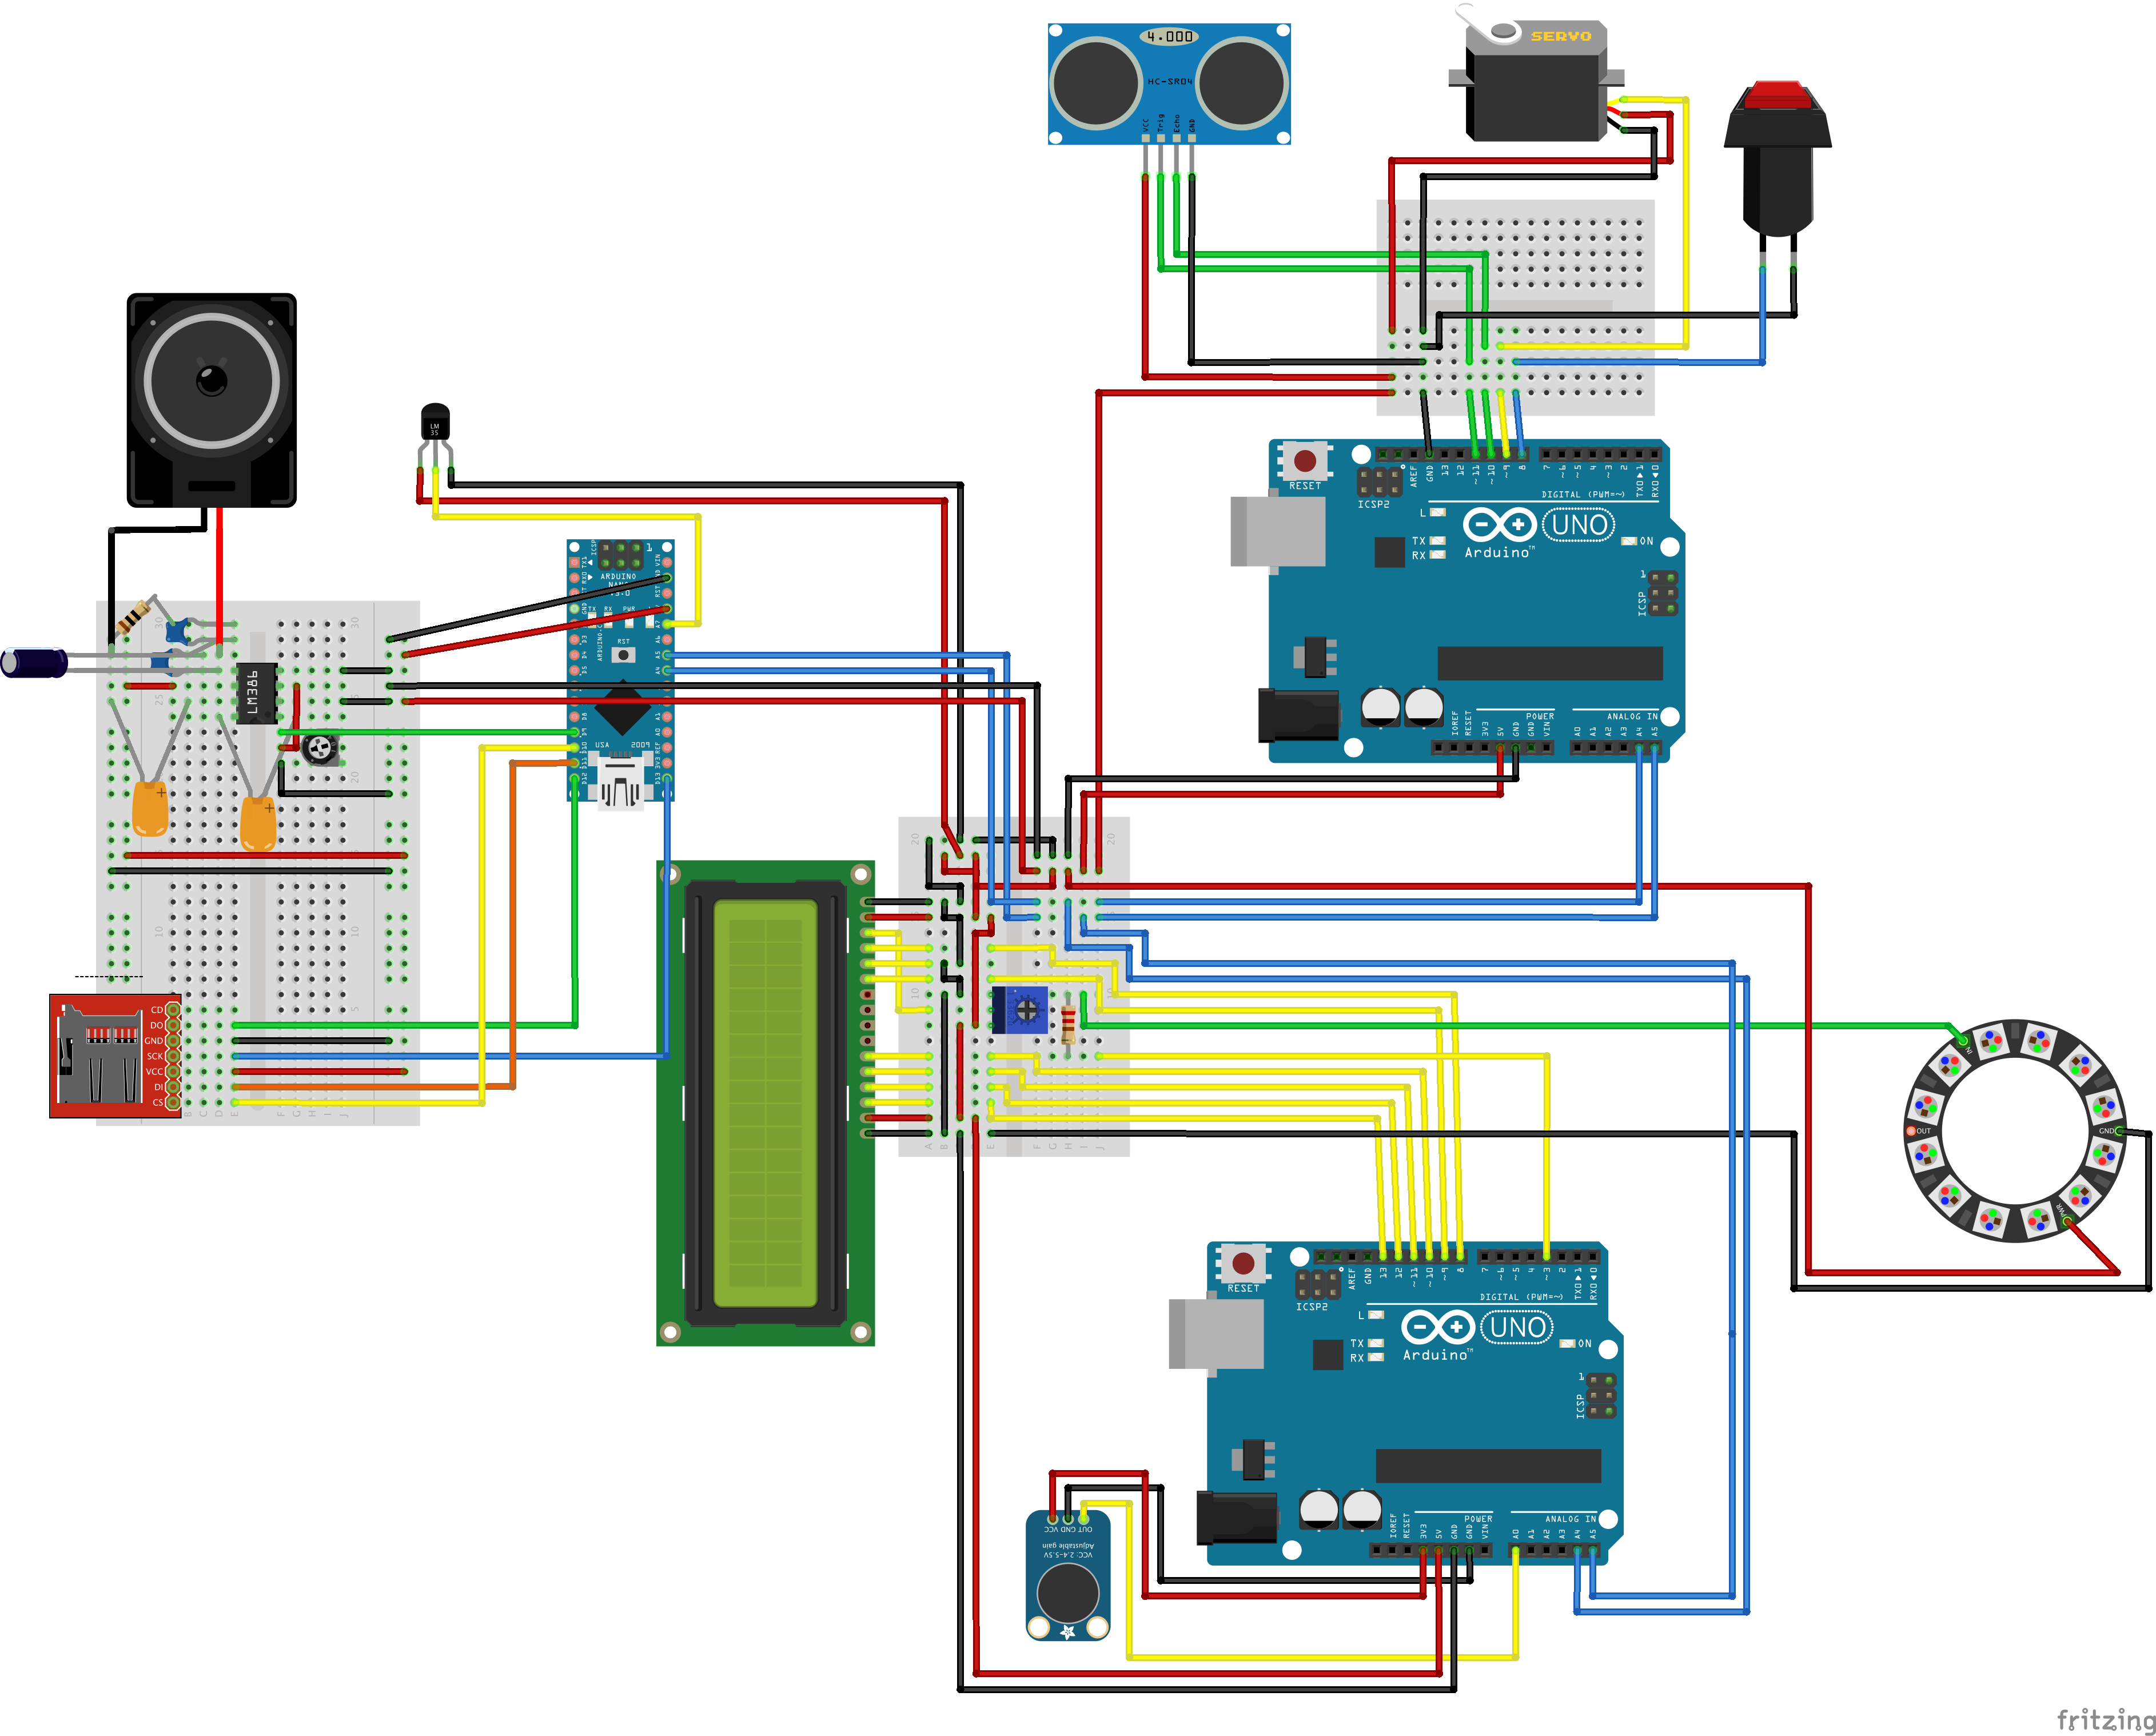
\includegraphics[width=0.7\textwidth]{robot_bb.png}\\
\textbf{Main Block Diagram}\\\\
\includegraphics[width=0.5\textwidth]{blockdiagrammain.png}\\
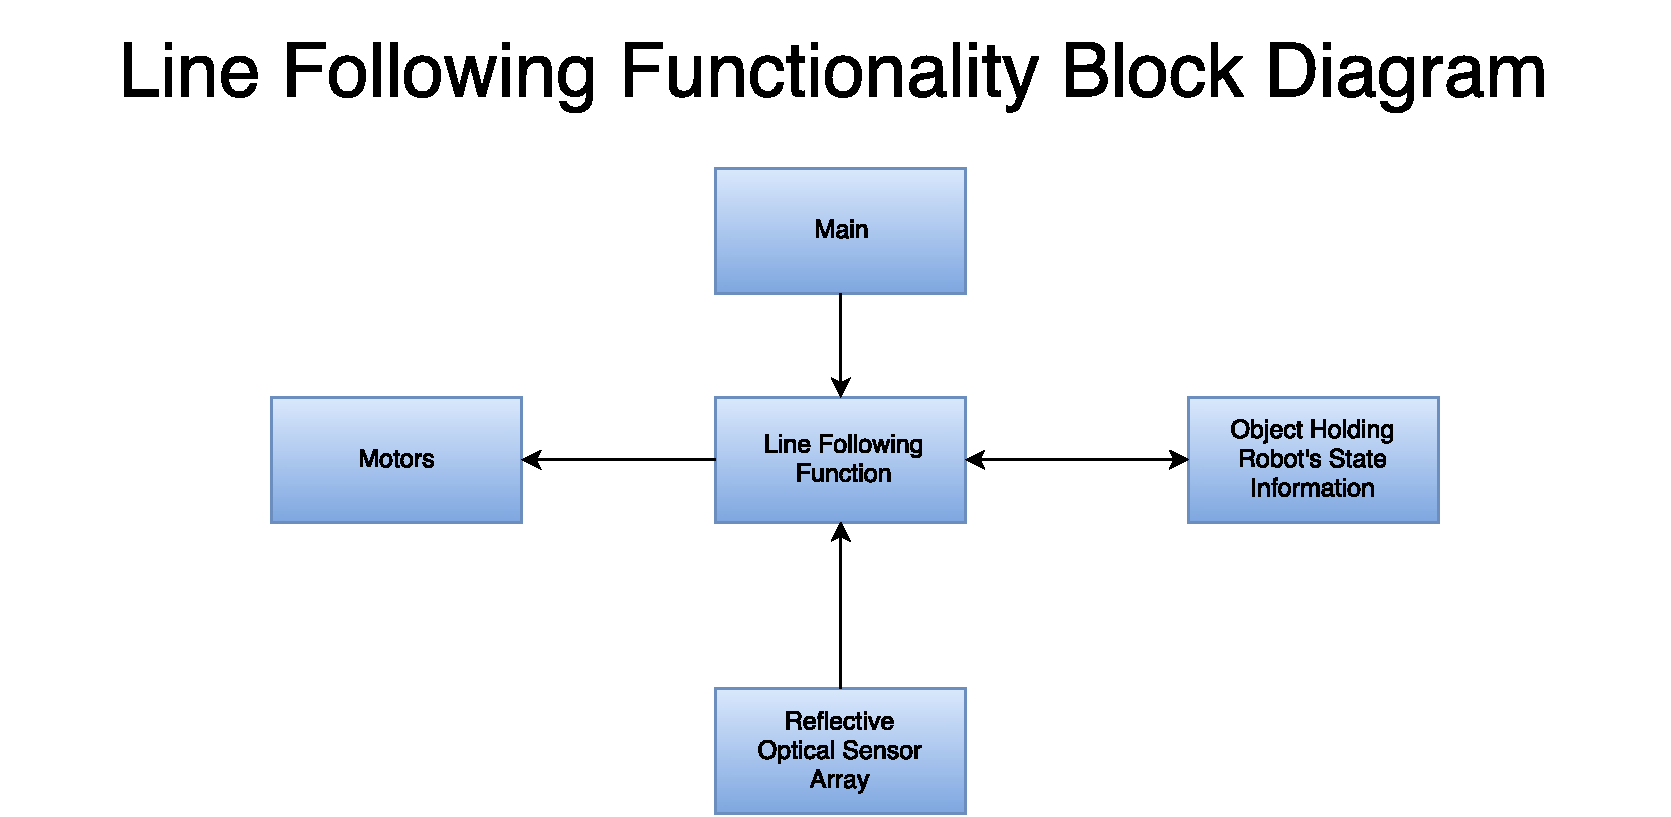
\includegraphics[width=0.5\textwidth]{line_following_block_diagram.pdf}\\
\textbf{Autonomous Mode Block Diagram}\\\\
\includegraphics[width=0.5\textwidth]{Free_drive_block_diagram.png}\\
\end{document}

